\documentclass[review]{elsarticle}

\usepackage{lineno,hyperref}
\usepackage{rotating}
\usepackage{algpseudocode,algorithm}
\usepackage{hyperref}
\usepackage{listings}
\usepackage{xcolor}


\lstset{
basicstyle=\small\ttfamily,
}
\graphicspath{ {./images/} }

\modulolinenumbers[5]

\journal{Future Generation Computer Systems}
\begin{document}
\lstset{language=Python} 
\begin{frontmatter}

\title{EvoSwarm: An Event-based Architecture for Multi-population Optimization Algorithms}

\author[itt]{Mario Garc\'ia Valdez}\corref{mycorrespondingauthor}
\cortext[mycorrespondingauthor]{Corresponding author}
\ead{mario@tectijuana.edu.mx}

\author[granada]{Juan J. Merelo Guerv\'os}
\ead{jmerelo@geneura.ugr.es}

\address[itt]{Department of Graduate Studies, Instituto Tecnol\'ogico de Tijuana, Tijuana BC, Mexico}
\address[granada]{Department of Computer Architecture and Technology, Universidad de Granada, Granada, Spain}

\begin{abstract} 
Splitting a population into multiple instances is a technique that has
been used extensively in recent years in order to help improve the
performance of nature-inspired optimization algorithms. Work on those
populations can be done in parallel, and they can interact asynchronously,
a fact that can be leveraged to create scalable implementations based
on, among other methods, distributed, multi-threaded, parallel, and
cloud-native computing.  However, the design of these cloud-native,
distributed, multi-population algorithms is not a trivial task. Coming
from monolithic (single-instance) solutions, adaptations at several
levels, from the algorithmic to the functional, must be made to
leverage the scalability, elasticity, (limited) fault-tolerance,
reproducibility, and cost-effectiveness of cloud systems while, at the
same time, conserving the intended functionality. Instead of an
evolutive approach, in this paper we propose to create from scratch a
cloud-native optimization framework that is able to include multiple
algorithms and use few parameters to work. This solution goes beyond
current state of the art via a framework that is able to support
different algorithms at the same time, work asynchronously, and also
be easily deployable to any cloud platform. We evaluate the
performance and scalability of this solution, together with the effect
other design parameters had on it; in particular, the number and the
size of populations with respect to problem size. The architecture and
the implemented platform is an excellent alternative for running
locally or in the cloud, thus proving that cloud-native bioinspired
algorithms perform better in their ``natural'' environment than other
kinds of algorithms, % Did we compare it to other kind of algorithms?
                     % If we didn't, this should go - JJ 
                     % Compared against GA and PSO and others from BBOB - Mario
                     % on the algorithm, not speedup 
and setting a new baseline for scaling and
performance in the cloud.
\end{abstract}

\begin{keyword}
Multi-population \sep Nature-inspired algorithm \sep Parallel Genetic Algorithms \sep Cloud-Computing
\sep Event-driven architecture 
\end{keyword}

\end{frontmatter}

\linenumbers

\section{Introduction}

In the last decades, nature-inspired optimization algorithms have been successfully
applied to solve many complex real-world problems
\cite{yang2014nature}; these algorithms can be broadly grouped into evolutionary algorithms (EAs)
\cite{back1996evolutionary} and swarm intelligence (SI)
\cite{kennedy2006swarm}, as well as other categories; popular EAs
are Genetic Algorithms (GAs) \cite{holland1992adaptation,eiben2003genetic}, 
Genetic Programming (GP) \cite{back1996evolutionary}, Grey Wolf Optimization
(GWO) \cite{mirjalili2014grey} and Differential Evolution (DE) \cite{karabouga2004simple},
while examples of (SI) \cite{kennedy2006swarm} are particle swarm
optimization (PSO) \cite{clerc2010particle} and ant colony algorithms (ACO) \cite{dorigo1999ant}.

Besides being all population-based, they also share the common characteristic
of creating an initial set of random candidate solutions that are later used to
generate a new set of candidates, using a nature-inspired heuristic.
Population-based algorithms are intrinsically parallel, and can be implemented to run asynchronously.
The fitness of each individual can be (in general) evaluated independently of 
others, and similarly, each population could evolve in isolation. Researchers use the term
multi-population based methods when generally referring to techniques using
many populations as part of their optimization strategy. 
Since 
earlier works, researchers have been proposing some form of parallelization
\cite{muhlenbein1988evolution} to increase the scalability of these
algorithms that adds to this simple parallel execution some form of
interaction between the independently running populations.
The island model was one of the first techniques proposed for parallelization,
which led to an early proof of speedup   \cite{gorges1990explicit,grosso1985computer}. 
The concept was to divide a large population into communicated subpopulations. 
Since then, other population-based algorithms have adopted the concept, 
and researchers have found additional benefits
besides the execution speed; these include avoiding a premature convergence and
maintaining the diversity of the global population \cite{li2015multi}. 

Moreover, parallel implementations can run in two ways: synchronous and
asynchronous. When operations run in parallel but must maintain synchrony with
the other operations,  all operations need to finish to continue to the next
step. For instance, in a  master/worker model, the master needs to wait for all
workers to finish their operations before moving to the next iteration.  In
contrast, in an asynchronous execution,  operations are not synchronized with
each other, so there's no time lost waiting for other populations to
arrive to the synchronization point. Following the previous example, now the master operation can
continue to the next iteration, even if a worker has not finished its work.  In
the literature, we can find many asynchronous algorithms
\cite{coleman89,baugh2003asynchronous}, reporting benefits in execution time,
and scalability. In the particular case of asynchronous and cloud-native
multi-population algorithms, recent works propose an asynchronous communication
through a central repository \cite{sofea:cec2012, JSON} or message queues
\cite{salza2019speed, guervos2018introducing}, in this work we follow this
practice.

The trend concerning the parallel execution multi-population algorithms go from
earlier hardware-based implementations using transputers
\cite{gorges1990explicit}, multi-threaded \cite{merelo2019scaling}, and
multi-core systems \cite{Serrano2008,lai2019adaptive}. % many citations here - JJ 
And recently the focus has been on exploiting a higher number of processing
units by using GPUs \cite{tan2015survey,li2007efficient}, or distributed
systems; techniques used to achieve this include web-based \cite{JSON},
map-reduce \cite{fazenda2012},  grid \cite{munawar2010design,Gonzalez09},
voluntary computing \cite{MilkyWay}, and, more importantly, cloud computing
\cite{GValdez2015,salza2019speed,valenzuela2015implementing,FlexGP}. 

Cloud computing has become the standard way of running
enterprise applications, not only because of the convenience of the
pay-as-you-go model or the non-existent cost of physical facilities, but also because
it offers a way of describing the infrastructure as part of the code, so that it
is much easier to reproduce results and this has been a boon for scientific
computing.  However,  cloud computing has also been evolving, going from simply
putting using virtual machines elsewhere than on premises old-style monolithic applications, that is, applications
built on a single stack of services that communicate by layers, to microservices
\cite{microservices} and serverless architectures \cite{varghese2018next,Varghese2018849} that favor the parallel and asynchronous communication of
heterogeneous resources; in the process, a new process for designing {\em cloud
native applications} has been created, with brand new methodologies and
techniques \cite{Baldini2016287}. In these architectures, services or even
functions are seen as single processing points, departing from the monolithic
and even distributed paradigms, become a loosely coupled collection of {\em
stateless functions} \cite{malawski2017serverless}, that react to events and
only come into existence while they are doing some processing.
Systems developed with the patterns outlined above have the
properties of a reactive system \cite{boner2014reactive} and they are commonly
more flexible, loosely-coupled, and scalable. % Some properies and reference - Mario  
% Again, you have to justify the need for a reactive architecture and define it before this paragraph - JJ


When designing efficient multi-population algorithms, researchers need to
consider additional issues \cite{Ma2019}. These include the number and size of populations,
the interaction between them, the search area of each population, and the search
strategy and parametrization of each population. We must take into account
these high-level issues when designing a parallel architecture. Researchers 
and algorithm designers willing to  adapt to the cloud their
multi-population solutions face the additional challenges:
\begin{itemize}
    \item They need to change their current solutions to a reactive architecture in which processes
    communicate with each other by exchanging messages asynchronously and react
    to a continuous stream of data. One of the options is to consider
    populations as messages to be modified asynchronously by functions. 

    \item To scale the system, when it is possible, they must use stateless functions for
    processing. 

    \item They need to establish a workflow of local development and prototyping while having the 
    option of deployment in a cloud provider. It is desirable to use modern development methodologies and technologies. 

    \item They must log experimental results and be able to replicate the experiments. 

    \item They must consider additional parameters that can affect the monetary cost or the performance of the
    execution — for instance, the format and size of messages, the number of
    worker processes and their capabilities.  
\end{itemize}

Taking these factors into account, in this work, we present EvoSwarm, 
a container-based application that reactively processes
isolated and
% Maybe container-based? You can create containers with podman - JJ
% yes, and is shorter - M
heterogeneous populations. The platform uses the Docker Compose tool for
defining and running experiments as multi-container applications. EvoSwarm is also released with a free licence in \url{https://github.com/mariosky/EvoSwarm}.
We preferred the use of a container-based application for this prototype because
it is more suitable for development and replication without the need for
additional components. Nevertheless, the application is compatible with other
orchestration and deployment technologies if more scalability is needed. 
With additional configuration settings, applications can be deployed 
to a Docker Swarm or a Kubernetes system.  

Docker container images host the stateless functions responsible for running 
a search strategy on several populations, these functions could also be ported
directly to a Function as a Service (FaaS) \cite{Roberts2016} implementation.
% Need to improve the next paragraph or maybe move it to another place - Mario
Researchers then define the configuration of services used by
a multi-population algorithm using a YAML file. Any researcher can deploy and
start all the services from this configuration file with a single command. Once
the services are up, multiple instances of an experiment can be sent to a queue
for their execution. The platform includes containerized services that are
compatible with other container orchestration technologies like Kubernetes and
Docker Swarm. The services included are a Redis Server used for the Message
Queue implementation and logging and an Experiment Controller implemented in
Python. Developers of population processing functions have the freedom to
implement new population-based algorithms or operators in the language they
choose inside a container, as they only need to subscribe to a channel of the
Message Queue and have the ability to read the population and parameters as JSON  
file.

This paper extends our earlier publication on the topic
\cite{guervos2018introducing}, and we highlight the main contributions as
follows:
We have proved that cloud-native applications are
able to easily accommodate multi-paradigm bioinspired algorithms
with little efforts of parametrization and
that a combination of algorithms has better speedup and performance
than any single one taken independently.

We have proved this in the following steps:
% The reviewer says that we should clarify the contributions, and the
% contribution should answer a research question. Maybe we should
% clarify these contributions to answer to that. Contribution should
% be something like "We have proved that cloud-native applications are
% able to easily accommodate multi-paradigm bioinspired algorithms
% with little efforts of parametrization and
% that a combination of algorithms has better speedup and performance
% than any single one taken independently.
% These items above could be preceded by "We have proved this in the
% following steps" - JJ
% I like it will put it just like that. 
% A reviewer also put enphasis on the workflow and reproductivility 
% and extracting a Model? we can put something on that too.

\begin{itemize}
    \item First, we present the design and implementation of a reactive 
    container-based application for the asynchronous execution of multi-population 
    algorithms. The source code and example container definitions are
    publicly available. % Not really a contribution. It's the mean to
                        % achieve the contribution - JJ
    \item Second, we propose a method for the deployment and execution of 
    multiple experiments by specifying the infrastructure as part of an 
    experiment definition in both local or cloud environments,
    facilitating the reproduction of experimental results. % Not clear
                                % what the contribution is. If this
                                % has been used for the first time in
                                % an EA environment, it should be
                                % stated that way. If not, it's also a
                                % mean to achieve the contribution - JJ
    \item Third, the application is compatible with the COCO benchmark 
    framework, allowing researchers to compare the performance of their 
    algorithms with other works. % Not really a contribution, but an
                                % implementation detail. Convenient,
                                % but does not advance the state of
                                % the art - JJ
    \item Fourth, we present an empirical study to validate the 
    applicability of our application,  measuring the execution time and  
    speedup.
    
    \item Lastly, we present a comparison between homogeneous and an ensemble of 
    multi-populations, using Genetic Algorithms (GAs) and Particle 
    Swarm Optimization (PSO) in a benchmark for the optimization of 
    continuous functions. % "Validate the applicability" falls short
                          % of being also a contribution. It must
                          % advance the state of the art, in which way
                          % does it advance? Speed (needs to be
                          % proved) Convenience (needs to be proved
                          % too) Scalability? (needs to be proved
                          % also). - JJ 
\end{itemize}

The organization of the paper is as follows: First, in Section \ref{multi}, we present a
background of the fundamental issues of integrating nature-inspired optimization
and multi-population methods. Section \ref{soa} presents state of the art relevant to
our work. In Section \ref{method}, we present the proposed method and the container-based
application in Section \ref{docker} .  Section \ref{setup} describes
the design of the empirical evaluation we designed to assess the effectiveness
of the method, and in Section \ref{results}, we report and discuss the results. Finally, we
offer the conclusions of this paper and suggestions on future work in Section \ref{conclusions}.


\section{Multi-population methods} % Is this part of the state of the
\label{multi}
                                % art? - JJ
% This the Background for the design decisions, but I think is also needed
% to better understand the state of the art.
% I don't know. Maybe it should be directly merged with the state of
% the art, if there's some essential to our paper it should go to the
% introduction - JJ

% Also, multipopulation design of what?x
Multi-population based methods divide the original population into
smaller populations or islands, with every population carrying out the
algorithm independently, with synchronous or asynchronous communication with the
rest of the islands \cite{Ma2019}.% exemplify how this is done in different
                     % metaheuristics, especially those we will be
                     % using here - JJ
This relative isolation helps in maintaining an overall
diversity since each population will search in a particular area, at least
between communications. The recombination mentioned above (mixing) or migration
between populations is needed to avoid a premature convergence of candidate
solutions since smaller populations are known to perform better for a given
problem than bigger populations \cite{li2016multi,wu2016differential}. % Smaller populations converge
                                % prematurely or perform better? - JJ
However, it gives them the added advantage of
parallel operation. Additionally, and in some cases, multi-population algorithms
scale better than expected due to the interaction between the algorithm and the
parallelism of the operation \cite{ALBA20027}. % Need to clarify this
                                % and if it extends to Swarm
                                % algorithms too
                                % Also, is your objective to achieve this superlinear speedup? - JJ

However, in most cases, algorithms applied to each population are
homogeneous, or at any rate, the same variant of the algorithm. As long as this
parallel operation is not synchronous, other population-based algorithms, or, as
a matter of fact, any algorithm, could be easily integrated. That is why several
works based on multi-population are heterogeneous, integrating various
optimization algorithms, and often performing better than single-population or
homogeneous optimization algorithms \cite{wu2016differential,nseef2016adaptive}.

Heterogeneous algorithms add another degree of freedom to the problem of finding
the correct parameter settings for an algorithm; because some parameters affect
the accuracy of the solution and the convergence speed of the algorithms as they
tip the balance between exploration and exploitation of the search space. On the
other hand, current studies show that by having a high number of populations
interacting in parallel, the effect of the individual parameters of each
population is compensated by those selected in other
populations \cite{li2016multi,tanabe2013evaluation}. % reference - JJ

%%%%% ----------------- This gets lost in this section -----------------------------
In this work, we will use random settings within a specific range as results have shown
this is a valid solution to this problem \cite{garcia2014randomized}. % This should have been
                                % mentioned in the introduction - JJ

%%%%%% -------------------- This too. Should go up, to intro, or down,
%%%%%% to method - JJ
Some parameters, specially the population size, are
kept fixed in order to control more easily the execution of the algorithm. For
instance, by having the size of populations fixed, it is easier to control
the number of evaluations and the communication costs, when the algorithm is in
operation. % And to keep them more or less synchronized, which can be
           % interesting, too... But this should go to the
           % introduction also - JJ

%%%% ---------------------- Also to the introduction
Combining multiple algorithms, with different parameters, interacting with each
other at the same time, can benefit from the strengths of each. For instance, a
genetic algorithm could find a promising global solution that is not optimal
while another algorithm, more suitable for a local search, finds the global
optimum. This approach has been followed extensively in recent years with
success \cite{li2015multi,godio2016multi,biswas2014co}. 
Moreover, there is a need for frameworks, architecture, and
implementation models that can allow researchers the development of new
parallel, asynchronous, heterogeneous, and parameter-free algorithms in a scalable way.  

\section{State of the Art} 
\label{soa}

Although at first sight containers look like simply a method that
allows easy shipping of applications, they are much more than
that. One of the first features that make them interesting is their
ephemerality: fast startup and teardown time make them usable for
machine-independent and cloud deployment of simple, ephemeral and
maybe stateless functions. On the other hand, containerization also
allows, through the use of orchestration engines like Docker Swarm or
Kubernetes, or through simple, non-self-scaling specifications using
Docker Compose, a definition of all the relationships between
different parts of the application, or services. The full realization
of Docker-based architectures has led to the creation of a series of
patterns that, together, conform cloud-native application development
\cite{kratzke2017understanding}.

However, in the field of evolutionary algorithms, this has been a slow
realization, from the origins where Salza and Ferrucci
\cite{salza2016approach,salza2016develop} proposed an architecture
that carried evolutionary algorithms to the cloud, and which were
developed further in their next paper \cite{de2017parallel}. These
papers started to introduce cloud native aspects such as the use of
messaging queues and CoreOS as an operating system designed from the
ground up for container utilization in the area of evolutionary
algorithms. The way these containers are managed, however, is rather
classical in nature from the point of view of distributed EC: a
master-worker approach, communicated using RabbitMQ (a messaging
queue), where replicated workers perform the tasks in parallel. They
called their approach AMQPGA, inspired by the protocol, AMQP, used by
RabbitMQ, the messaging system. This classical approach has been also
followed by other authors by using other EA ``classical'' topologies
in the cloud: Dziurzanski et al. \cite{dziurzanski2020scalable} adapts an island model to
a container architecture, in a system that is functionally equivalent
to classical models, but with the added advantage of being easy to
deploy and run.

Later approaches use microservices \cite{khalloof2018generic}, or were
systematized \cite{salza2019speed} achieving speed-up through the
creation of an abstraction layer over the evolutionary algorithm
services, and also automation of the whole workflow. This research
bumped into some problems, since speedup is limited, mainly due to the
non-automatic scaling of services and also the presence of a single
master which is the one that runs the evolutionary
algorithms. However, this master-worker architecture can be turned
around with other kind of evolutionary architectures, such
as pool-based systems
\cite{valenzuela2015implementing,merelo2012sofea,sofea:cec2012} where
a better match to the inherently heterogeneous nature of cloud-based
architectures. Pool-based systems are closer to serverless systems
\cite{malawski2017serverless}, and they pull from the pool and run
whole algorithms, instead of just evaluation. The pool from where they
pull is the common store of results, and can be accessed in an
asynchronous way, which suits better the nature of cloud systems.


% a lot of this has been done in the previous method... Maybe there's
% not that much to do - JJ
% Hadoop 
%     Comparison \cite{ferrucci2018using}
%     Hadoop\cite{fazenda2012} 
%     FlexGP \cite{FlexGP}, 
%     elephant56 \cite{salza2016elephant56},

% Pool
%     SofEA \cite{merelo2012sofea,sofea:cec2012} , 
%     EvoSpace \cite{garcia2015evospace},
% Volunteer
%     evospace-js \cite{garcia2017evospace}
% Queue
%     Containers \cite{valenzuela2015implementing} \cite{salza2016approach} 
%     Seamless local and Cloud \cite{leclerc2016seamless}
%     Serverless KafKEO \cite{guervos2018introducing}, 
%     Docker Orchestation \cite{dziurzanski2020scalable,zhao2019cloud}
% PSO 
% PSO AWS \cite{li2015parallel}



\section{Proposed Method} 
\label{method} 

In this section, we present the design
and a container-based implementation of the model we propose for the execution
of multi-population based algorithms. We follow the requirements outlined in
Section \ref{multi} and the general design principles of cloud-native
applications we have mentioned earlier; our intention is to steer
clear of a direct translation of ``classical'' GA architectures to the
cloud and design from the ground up a cloud-native method. As a first step, we describe the general
architecture, and then  every component in detail. 

The most elemental data structure used throughout the system is the population; and at a higher
level, we can view the system as a continuous stream of populations
flowing from one process to the other. By ``continuous stream,'' we mean that ideally,
everything must happen asynchronously without components needing to wait for
others. In this kind of system, this streaming functionality is normally
implemented by using a message queue system. For instance, if one process needs
to communicate a population to another, it must pack the population into
a message, and then send the message 
to the queuing system without waiting for a response; this
means that after the process pushes the message, it continues its execution
without waiting for a result. On the other end, the recipient subscribes to the
message queue by defining an event handler method that is going to be triggered when a
message is pushed to it. The two components at each end of the queue are
Producers that push messages to the queue and Consumers that pull them. This
pattern is an essential component of a reactive architecture and makes
it 
highly scalable; one of the reasons for this is the use of functions
that have no secondary effects or access global storage, that is,
stateless functions. These functions do not need to read, keep, or modify data outside of the method. If
Consumers are implemented using stateless functions, and thus, there is no difference
between having one or many copies of the same function pulling work from the queue all at the
same time, because no side effects, including unwanted resource
locking problems,  are going to result from this concurrency.
% This is important and we should probably mention that in the
% introduction - JJ 
Based on these general principles we define next the proposed model.


\begin{sidewaysfigure}
    \centering
    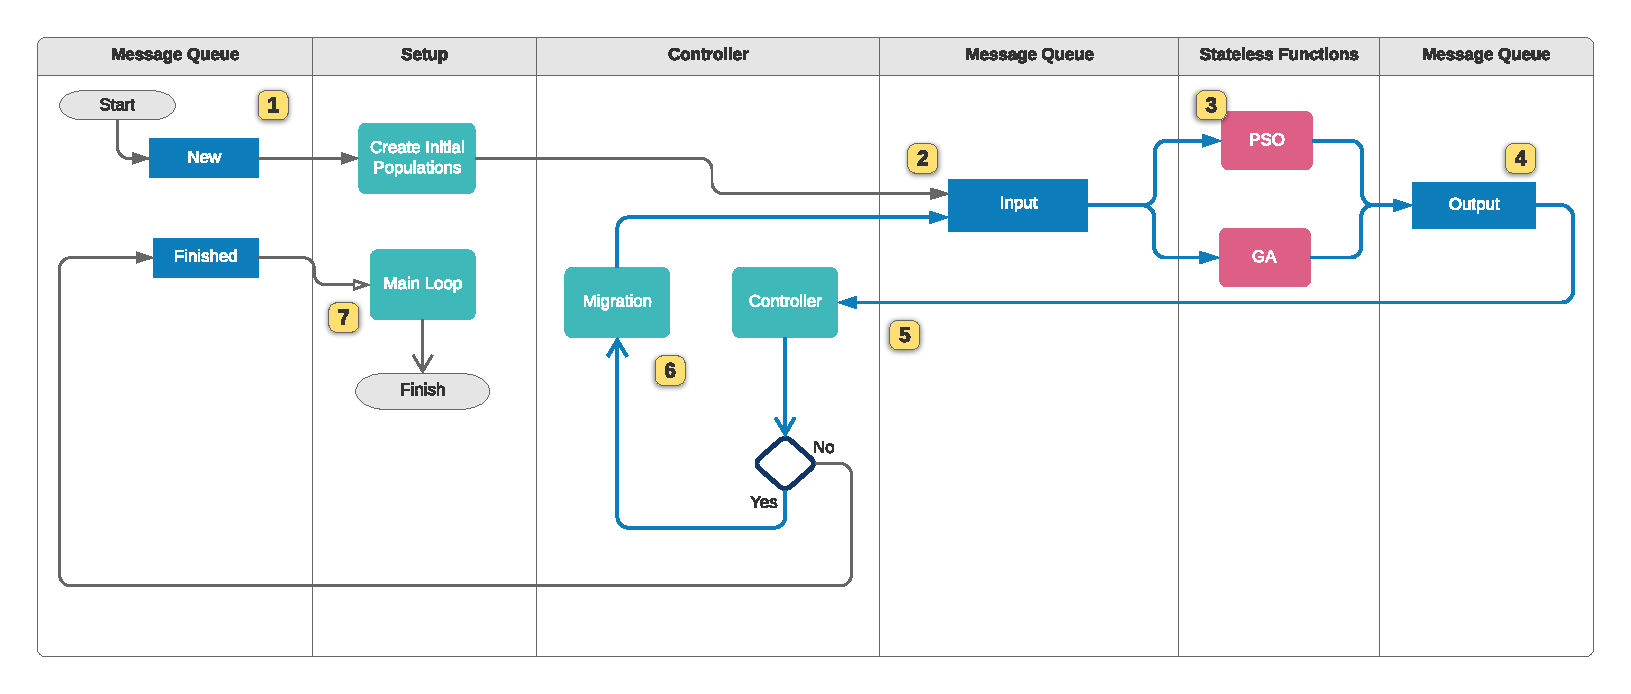
\includegraphics[width=\textwidth]{KafkEOsmall}
    \caption{The proposed general architecture, 
     showing each process in a swimlane, message-dataflow,
     message queues, and high-level tasks for each process.} 
    \label{fig:kafkEO}
\end{sidewaysfigure}

\subsection{Event Driven Model} 
\label{edm}
Based on a reactive architecture we proposed in a previous work
\cite{guervos2018introducing}, we now describe the general architecture shown in
Figure \ref{fig:kafkEO}. Again, we can explain the model using the analogy
of producers and consumers of messages. First, we can see that
there are two queues, one labeled \texttt{Input}, and the other one \texttt{Output}. In the diagram, 
push operations on a queue are represented by solid arrows connecting to the left side
of the queue box, and pull or pop operations as solid arrows leaving from the right side.
Also, the architecture has at least four processes indicated in the diagram as
swimlanes: First, the \texttt{Setup} process, responsible for the reading a configuration
file, and creating the initial populations. Second, the \texttt{Controller} process,
responsible for the migration between populations, and keeping track of the
iterations of the algorithm. The \texttt{Message Queue} process runs the \texttt{Input} and \texttt{Output}
queues. Finally, there is at least one \texttt{Stateless Function} process responsible
for running the isolated algorithms. In the example, two processes \texttt{PSO} and \texttt{GA},
are shown. 

The algorithm starts with the \texttt{Setup} process pulling a configuration message from
the \texttt{Experiments} queue, this is not shown in the diagram. The configuration message 
includes all the parameters needed to execute the algorithm, among other things,
the number of populations, the number of individuals, and the number of iterations
of the algorithm. We give more details about the configuration data structure
in Section \ref{experiment_flow}. % Missing  % added 
Once the configuration is read, we can follow the path of 
messages as follows:

\begin{enumerate}
\item In this step, the specified number of populations are created according to the 
parameters found in the configuration structure. The population at this moment is just
static data, including each individual inside. Each population includes a metadata
section where its algorithm and execution parameters are specified. For instance, 
for a GA, the mutation rate, type of crossover operator, and other values are indicated.

\item Each population is then pushed to the \texttt{Input} queue, so they can be consumed 
by Stateless functions responsible for the execution of the search.

\item One or more \texttt{Stateless functions} are constantly pulling population messages
from the \texttt{Input} queue. Taking the population data and metadata as parameters, these 
functions are responsible for the actual execution of the optimization algorithm. 
They take the current state of the population and run the algorithm for a certain 
number of iterations. 

\item Once they finish the execution, the population state
is packed again along with additional metadata about the execution of the algorithm.
The resulting populations are now pushed to the Output queue. Once finished, another 
population is pulled from the queue.

\item The \texttt{Controller} process is responsible for keeping track of the progress of 
the search. It pulls current populations from the \texttt{Output} queue, inspects the metadata 
and if an optimal solution has been found or the maximum number of iteration has been
reached it signals the stop of the execution. 

\item Otherwise, it passes the stream of messages 
to a migration process, where populations are mixed with each other. New populations 
are generated from this migration, and they are again pushed to the Input queue to continue 
in a loop. The \texttt{Controller} is also responsible of logging the metadata received with the
messages.  
\end{enumerate}

This reactive architecture has the following advantages:\begin{itemize}
\item 
An important aspect of proposal is the decoupling of the population and 
the population-based algorithm. It is common that in a classic island-based algorithm
each island is executed in a separate processing node, i.e. in a virtual machine, CPU,
or thread. In this case we can have just one processing node, or many nodes, each 
running a different search strategy, or using its own parameters. 
\item 
Also, the reactive controller gives designers more control over the multi-population algorithm.
In this process, designers can dynamically change the number of populations, population parameters,
and migration details on-the-fly.
\item 
Another advantage is that algorithm designers have many options for implementing this simple architecture. 
The same basic components can be implemented as a single multi-threaded program, or 
as a highly scalable serverless cloud application. Most modern languages include 
constructs for asynchronous programming using queues or channels, for a multi-threaded
execution.
\end{itemize}

\begin{figure}[ht]
    \centering
    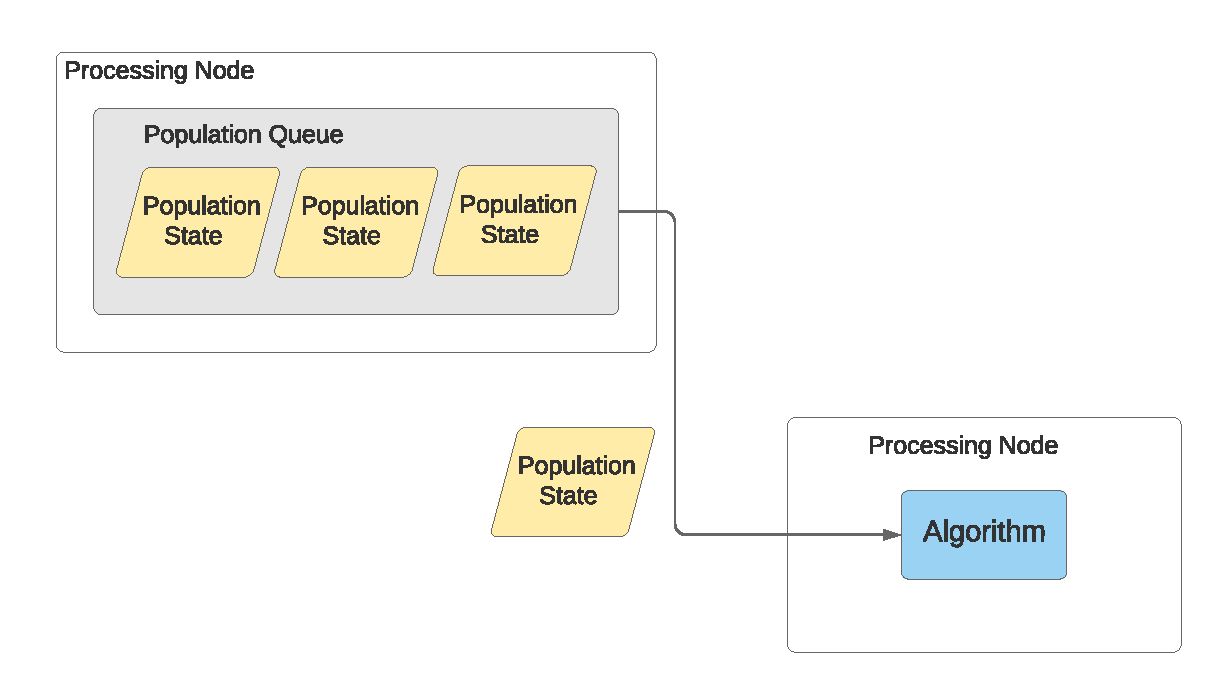
\includegraphics[width=\textwidth]{population_message}
    \caption{Population State and dataflow between processing nodes of a message-based algorithm.}
    \label{fig:population_message}
\end{figure}

On the other hand, there are several caveats as well:
It is more costly to move entire populations as messages than only passing certain individuals 
from a process to another. Designers must consider this cost when working with large
individuals, and if possible send populations using several messages, use compression or 
adjust the size of populations. Pool-based algorithms also suffer from this drawback, but 
web based implementations have been working with continuous optimization problems of 1000 dimensions.
But, in other cases this is not a viable approach. 

\begin{figure}[ht]
    \centering
    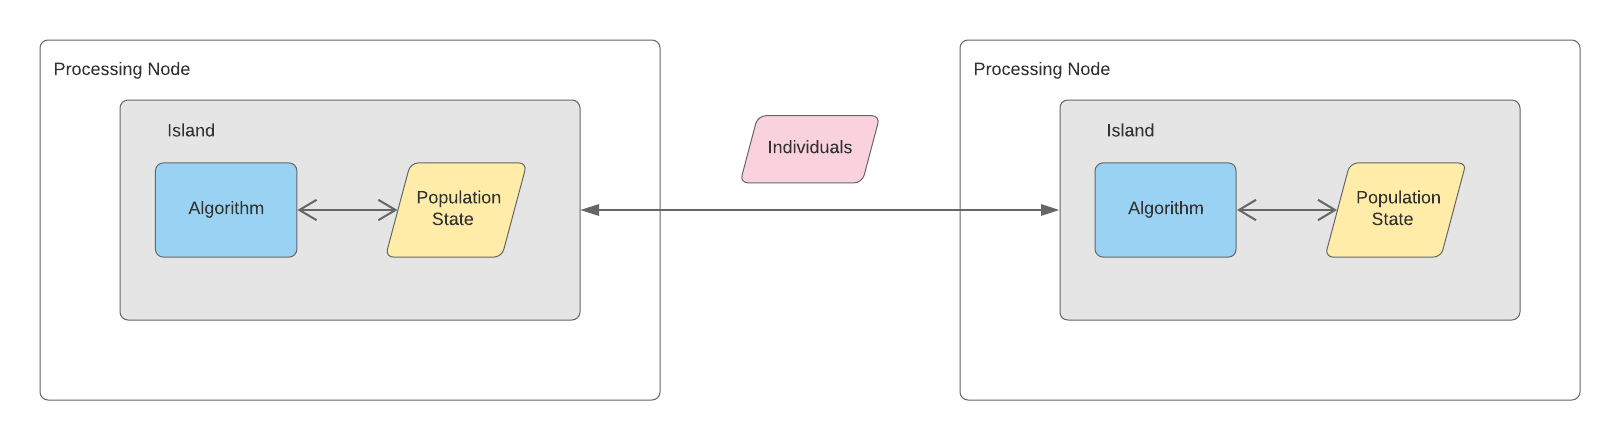
\includegraphics[width=\textwidth]{classicisland}
    \caption{ Population State and dataflow between processing nodes of a classic Island-based multi-population algorithm. }
    \label{fig:classicisland}
\end{figure}

\subsection{Comparison with other cloud-based works} 
\label{comparison}

Next, we compare the message-driven architecture we presented against four other
proposals for multi-population algorithms found in the literature. We center the
comparison on the coupling and communication between the main components:
populations, processing nodes, and algorithms.  In Figure \ref{fig:population_message} we show the
main components of a message-driven architecture. We can see that the algorithm
and populations are separated, and the \texttt{Population queue} keeps the state
of populations. While algorithms only need the populations as parameters
for their execution.

% We need to add references to the respective papers - Mario

In contrast, in the classic island model shown in Figure
\ref{fig:classicisland}, algorithms are  population methods, and the same processing
node keeps both the algorithm process and the state of the population.  Other
processing nodes follow the same configuration and form of execution, and they
only pass specific individuals between them.  In this model, adding additional
processing nodes, on-runtime, can be more difficult, because they need to have
an addressing mechanism or simply be aware of these new nodes. This is
solved in part in Peer to Peer (P2P) evolutionary algorithms
\cite{juanlu:europar}, but coupling still exists, meaning that every
node must run the whole evolutionary algorithm and hold full copies of
its subpopulation. 
% JJ, help I don't know if this is clearly understood, a mean like a
% DNS - Mario
% Added something - JJ

\begin{figure}[ht]
    \centering
    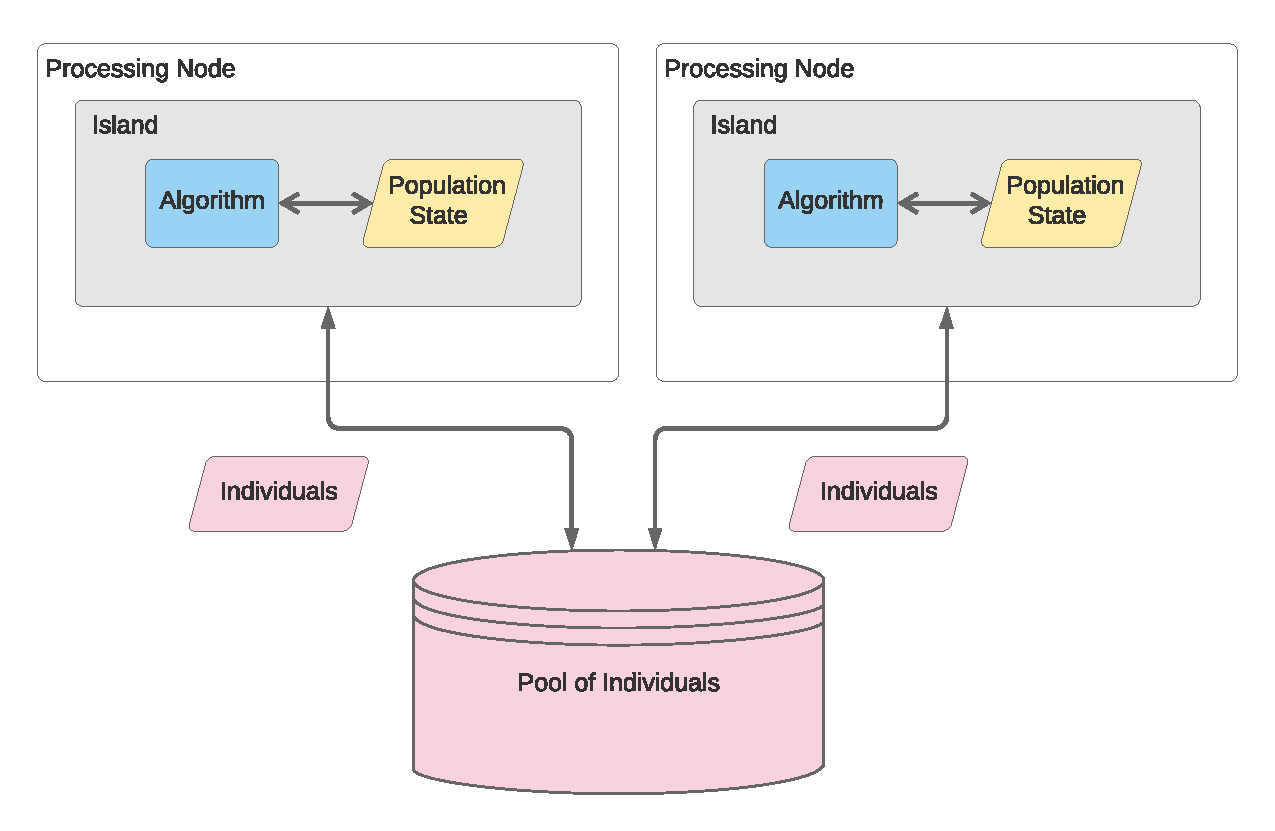
\includegraphics[width=\textwidth]{pool_island}
    \caption{Population state and flow of data between processing nodes of a Pool-based multi-population algorithm.}
    \label{fig:pool_island}
\end{figure}

A typical design pattern used to alleviate the above drawbacks is the use of a
central repository or pool of individuals that is available to all processing
nodes.  In Figure \ref{fig:pool_island} we show the main components of a pool-based
multi-population algorithm. Although algorithms and population state remains
coupled, now, processing nodes do not communicate directly with each other.
Instead, they interchange individuals with the pool. Communication between nodes
is not affected if the system adds or removes nodes because they do not know
about each other.  Since the state of the global population is stored in
external processing nodes, the system needs additional communication and
processing for keeping track of each population.

We show another pool-based approach in Figure  \ref{fig:population_pool}. In
this design, the global population is stored in a central repository, while
isolated algorithms take random samples of the global population and use this
temporal population as parameters. An advantage of this design is that the
sampling provides a type of migration between isolated populations. A problem
found is that when a processing node returns a population to the pool, the
state of the population is lost. But having the algorithm decoupled opens the
possibility of implementing the system using serverless functions.

\begin{figure}[ht]
    \centering
    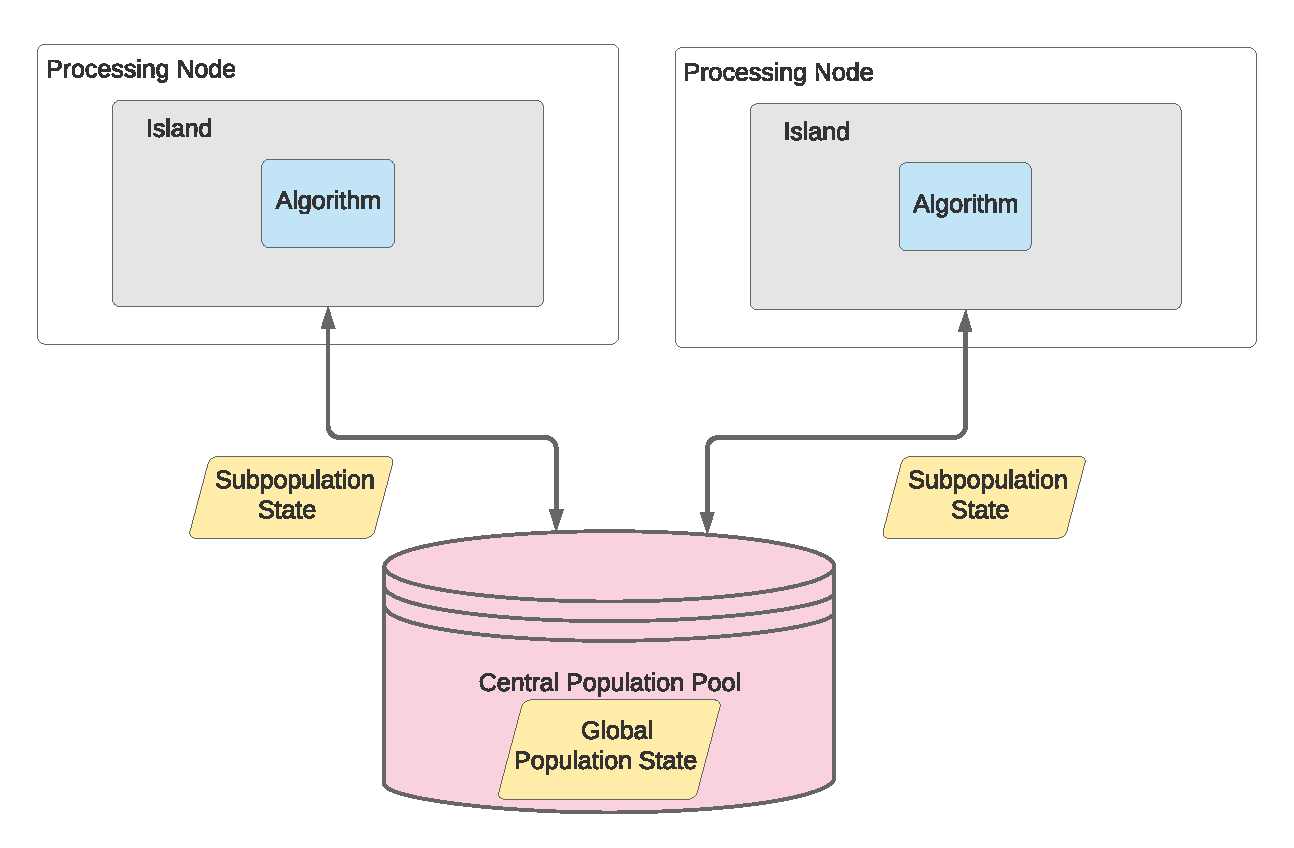
\includegraphics[width=\textwidth]{population_pool}
    \caption{Population State and dataflow between processing nodes of the EvoSpace algorithm.}
    \label{fig:population_pool}
\end{figure}

\section{Container-based application} 
\label{docker}

We have mentioned several advantages of a cloud-native application for running
multi-population based algorithms, but there are in our experience several
practical issues of this approach. In general, cloud platforms have free-tiers
for their services, and many offer academic discounts to students. But once we
pass to the pay-as-you-go tier, computing resources need to be
managed, and, where possible, its cost minimized.  First,
in many cases,  a credit-card is needed to guarantee the payment of the
resources consumed and someone responsible for assigning quotas and, more
importantly, special keys for using the cloud's API.  If these keys are
compromised or shared by their holders,  additional costs or administrative
procedures are in order. For those cases when a prototype platform is needed,
for instance, students developing a new algorithm variant or experimenting with
a published work, a container-based platform can be more practical. Container
technology enables researchers the local deployment of all the infrastructure
needed to run the experiments. Later, if needed, the same system could be
deployed to the cloud.

% The main advantage of container deployments over virtual machine
% instances is that they add much less overhead to communication between
% them, and they are much more economical to deploy. Scaling and
% monitoring can be done much more easily through cloud orchestration
% systems such as Kubernetes; these are the reasons why we chose it for
% this work.
% I don't see this line of argument. You can do exactly the same with
% virtual machines instead of containers. Also, you can test a virtual
% infrastructure locally and then only when it's needed deploy it to
% the cloud. If you want to give good reasons for using containers
% instead of virtual machines, there are quite a lot non-economic ones
% - JJ
% OK, I will add an issue - Mario
% Did you finally? - JJrehe
% I did not, will add and assign it - M
There are many advantages of container-based architectures over one
based on virtual machines. The main ones are architectural: it makes
the design of an application gravitate towards a set of decoupled
tasks, that use reactive, event based programming, to interact with
the rest of the application; containers hold micro-services that are
much easier to test, integrate and deploy. It also simplifies
the interaction APIs. Of course, that makes them more economical in a
pay-per-use cloud provider, but that is not the main reason why we
have chosen them in this paper; reproducibility of experiments and a
clear and idempotent description of the architecture through docker
compose are the main reasons. 

In this section, we propose a design of a reactive container-based application
for executing multi-population based optimization experiments.  For the design,
we followed the design patterns highlighted in the previous section, and again
we can go back to Figure \ref{fig:kafkEO} and use it as a guide for explaining
the main components and their interactions. 

% But first, we give a brief description of the technology we used. 

% Add if needed
%\subsection{Containers} 
%\label{containers}
% TO DO

%\subsection{Docker Compose} 
%\label{compose}
% TO DO
 

% Do we need a description of every container? Wouldn't a general 
% description  of the containers used be enough? - JJ 
% Ok, I thin only workers and the controller need to be described in detail - Mario 
\subsection{Message Queue Container} 
\label{message_container}

In this work, we implemented all message
queues in the Redis memory store. Early cloud architectures
\cite{de2017parallel} used queues for communication, although in that
case RabbitMQ was the chosen tool. Redis is faster, and also can act
as a data store from where we can control the state of the application.
Each queue is a Redis List object, and we use
the \texttt{LPOP} (left pop), and \texttt{RPOP} (right pop) commands for a queue like behavior.
In those cases where we needed a blocking behavior, i.e., when a process needs
to wait until a message is available, we used the blocking versions \texttt{BLPOP} and
\texttt{BRPOP}. Redis in-memory operation are very fast, and all of the above 
operations have a time complexity of $\mathcal{O}(1)$. We use the official 
\texttt{redis:alpine} container image from DockerHub.  

\subsection{Controller Container} 
\label{controller}

The controller is an essential component of the architecture (see Figure \ref{fig:kafkEO})
because it is responsible for maintaining the evolutionary loop. It takes newly
evolved populations from the \texttt{Output Queue}, mixes them,   and produces new
messages from the result. At the same time, it must keep track of two conditions
for ending the loop: the number of messages it has received reaches a maximum
value, or the error of the best solution goes below a specific threshold.  Finally, it
must filter out remnant messages from other experiments. Messages from other
experiments can remain in the queues because of the asynchronous nature of the
system.  We chose to implement the controller in Python but using an API
specialized in asynchronous event-driven programming over data streams.  
The open-source library is called Reactive Extensions (ReactiveX) for Python 
\url{https://github.com/ReactiveX/RxPY} an it is based on the Observer 
pattern \cite{gamma1995design} and functional programming.

\begin{figure}[ht]
    \centering
    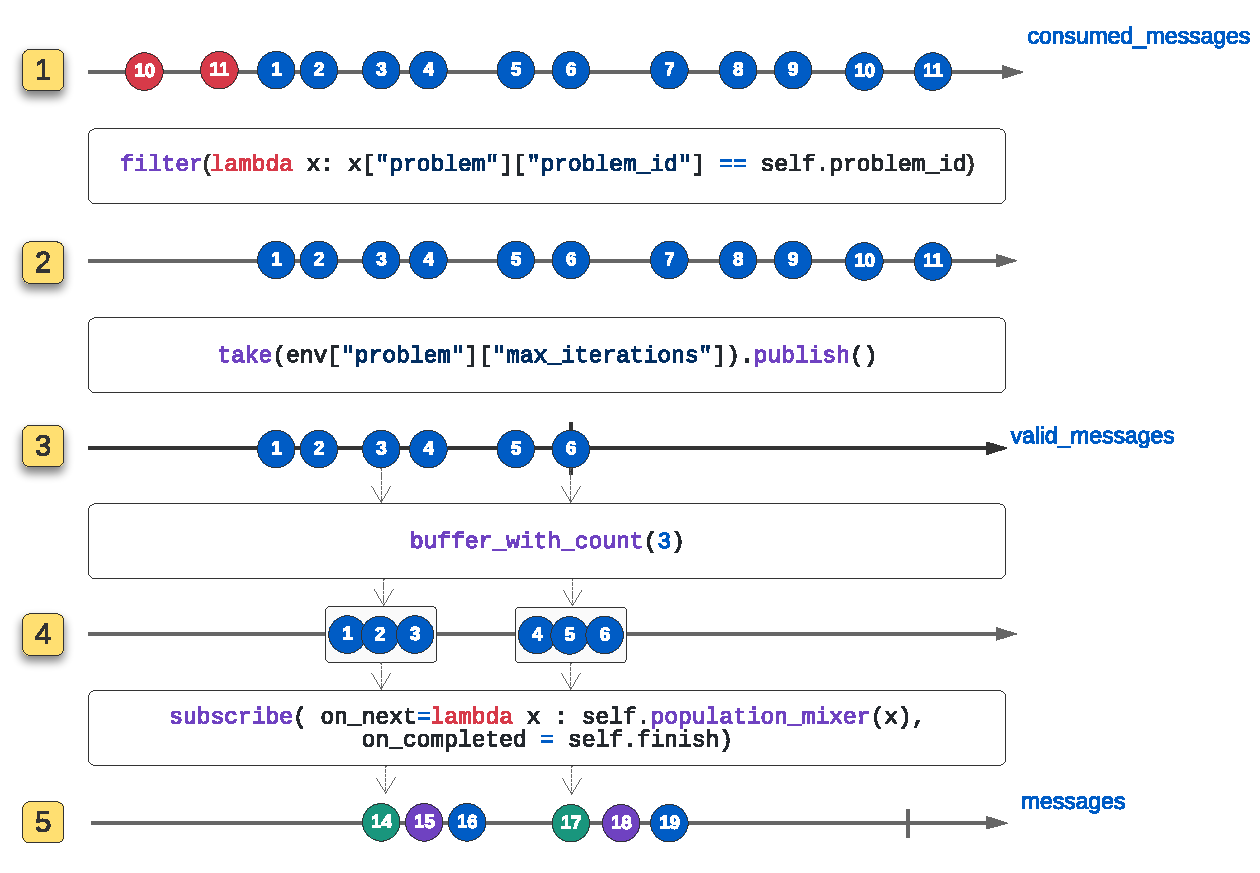
\includegraphics[width=\textwidth]{marble_controller}
    \caption{Marble diagram for the Reactive Python implementation of the Controller}
    \label{fig:marble_controller}
\end{figure}

In ReactiveX, an \texttt{observer} object subscribes to an \texttt{Observable} instance. 
Observables emit a sequence of items, and all the subscribed observers react to each emission. The
ReactiveX library includes several reactive operators that we can use to
transform and combine sequences of items. These operators provide reactive
extensions that allow us to compose asynchronous sequences together in a
declarative manner. In Figure \ref{fig:marble_controller}, we use a marble diagram to
represent the composition of \texttt{Observables} and reactive extensions operators. We
represent the timeline of an \texttt{Observable} as a horizontal arrow, which indicates
that time flows from left to right. In the diagram, items are represented as
marbles. The position of each marble indicates the point in time when they were
emitted by the \texttt{Observable}. Reactive operators are represented as text boxes,
showing the transformation to be applied. Normally, a transformation results in
another \texttt{Observable}, again emitting new results.  For asynchronous programming, 
this approach is more elegant than nested callbacks, that are more difficult 
to code and debug. 

Now we proceed to explain the reactive implementation of the controller.
In Figure \ref{fig:marble_controller}, we  have the following composition of Observables:

\begin{enumerate}
\item The controller continually pulls new messages from the \texttt{Output} 
message queue. These messages are instantly emitted by the  \texttt{consumed\_messages}
\texttt{Observable}. In this particular period, we can see that the stream receives 
two populations from another experiment, and are shown as two red marbles.  
The filter operator removes all messages that belong to a different experiment; 
in this case, we are only interested in blue marbles. 

\item The \texttt{max\_iterations} parameter indicates the number of populations that
are going to be accepted. When this number of messages is reached, we must
end the loop. In this example, \texttt{max\_iterations = 6},  the take operator 
assures that only 6 messages are received. After the \texttt{Observable} emits 
the sixth message, it triggers the completed event.

\item Many observers can be subscribed to the \texttt{valid\_messages} \texttt{Observable} because it
emits all the valid items. At the moment, there are to additional methods
subscribed that we are not showing, one for logging and the other for monitoring
the search.

\item The   \texttt{buffer\_with\_count(3)} operator, waits until it receives 
three valid messages to emit a single message that contains a list with
the previous three. The \texttt{population\_mixer}  method requires that list to mix them. 
In our previous work, we needed a local buffer for storing a certain 
number of populations to mix them with others. This design has the advantage
of not needing extra memory, and it integrates better with the reactive paradigm.
A possible disadvantage can be that it only mixes contiguous populations,
but this can be mitigated with a larger buffer.

\item The \texttt{population\_mixer} receives a list of three populations,
let us say [A, B, C], and calls the migration method shown in
Algorithm \ref{alg:migration}  for [A, B], [B, C] and [A, C]. 
The migration algorithm sorts both populations and generates
a new population containing the best half from each.
This migration method is similar to those used successfully in previous 
works on pool-based algorithms \ref{fig:pool_island}.  
Finally, the method pushes the new populations to the 
\texttt{messages Observable}. From there, a
\texttt{publish(population)} observer is responsible for pushing
the newly generated populations back to the \texttt{Input} message queue.
\end{enumerate}

\begin{algorithm}
    \caption{Migration}
    \label{alg:migration}
    \begin{algorithmic}[1]
        \Procedure{cxBestFromEach}{$pop_1,pop_2$}
            \State $pop_1.sort()$
            \State $pop_2.sort()$
            \State $size\gets min(len(pop_1), len(pop_2))$
            \State $cxpoint\gets (size-1)/2$
            \State $pop_1[cxpoint:]\gets pop_2[:cxpoint+2]$
            \State \textbf{return} $pop_1$
        \EndProcedure 
    \end{algorithmic}
\end{algorithm}



In the next section, we follow the algorithm flow and describe the 
implementation details of the \texttt{worker} containers. 

\begin{figure}[ht]
    \centering
    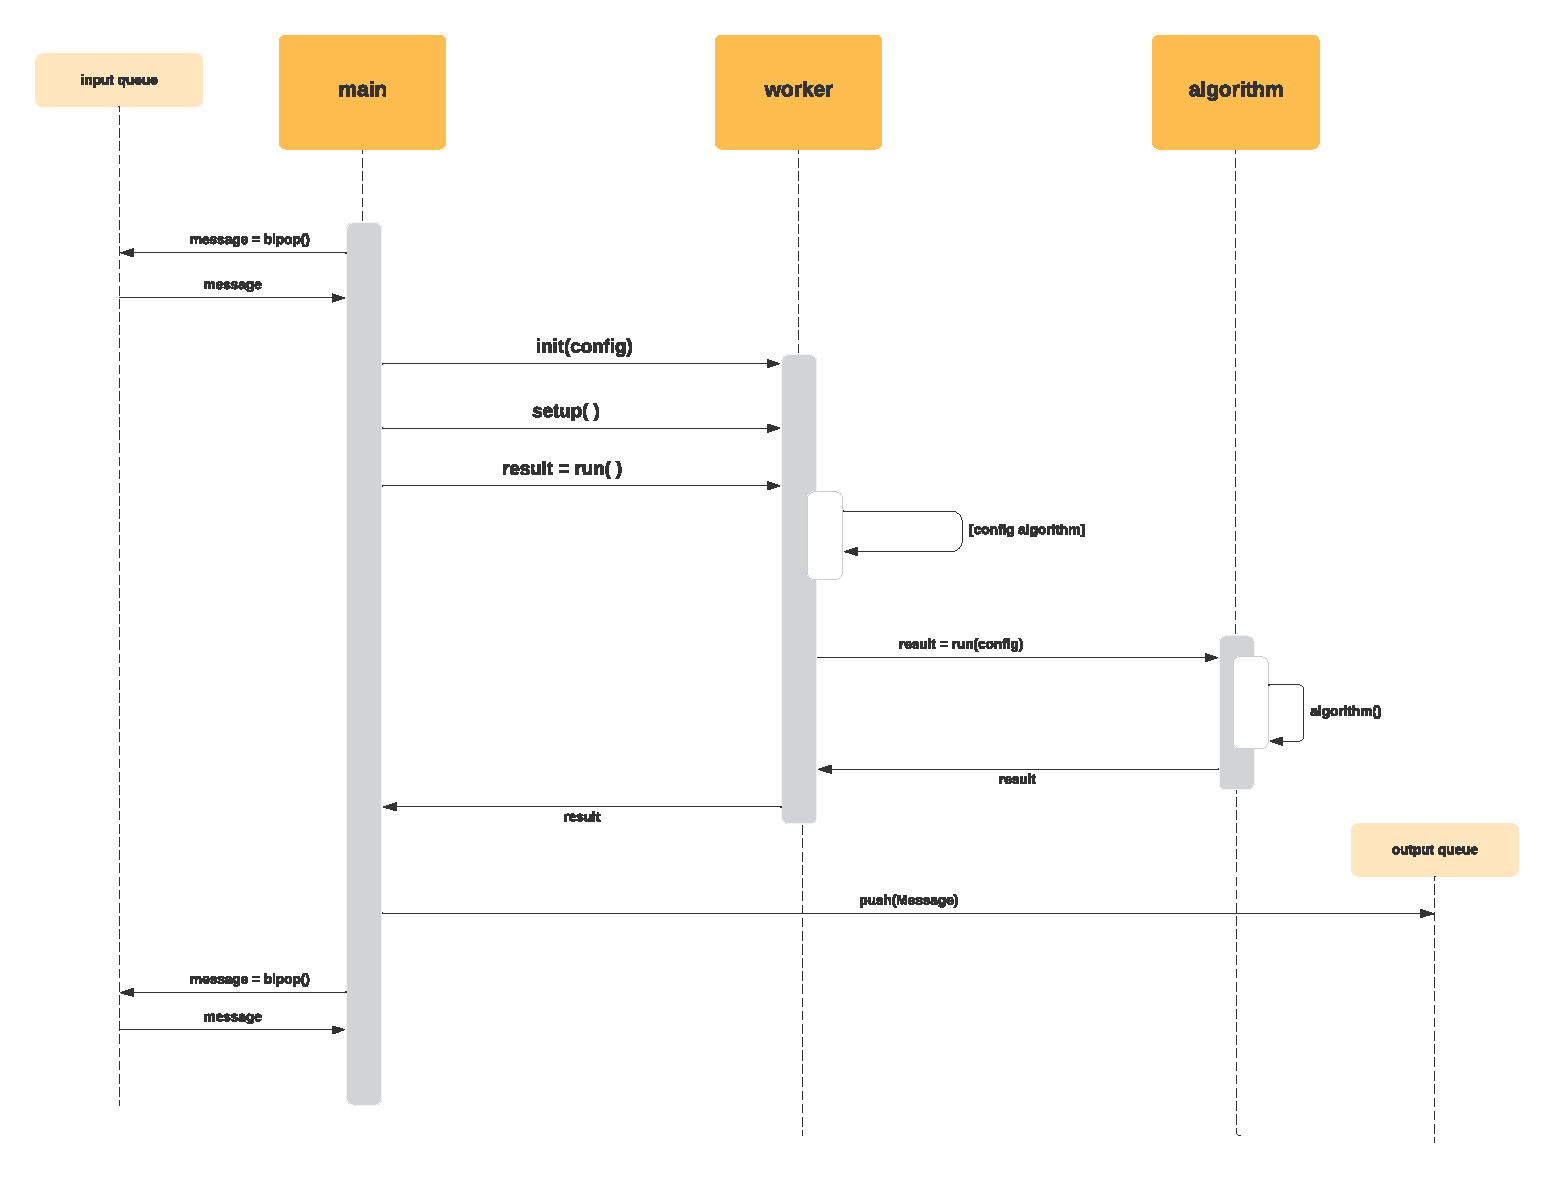
\includegraphics[width=\textwidth]{worker_new}
    \caption{Serverless function implementation details. Showing the worker algorithm in each container}
    \label{fig:worker}
\end{figure}


% Maybe you should say here how everything wors: launch with
% Docker-compose, whatever. That's the issue that one of the reviewers
% say - JJ 

% This issue is also commanted in the experimental section
% I will explain it and then we can see where it goes. - M  

\subsection{Worker Containers} 
\label{workers}

Worker containers include a Python script called \texttt{main.py} running an
infinite loop, continually trying to pull a new population to work on it. Once
\texttt{main.py} receives a message containing configuration data, it creates a
worker object responsible for initializing and running the specified stateless
function (i.e., GA or PSO) with the population and configuration in the message.
Once the function returns the evolved population, the
the main script pushes the results to the \texttt{Output} queue, and continues
the execution to the infinite loop. This process is shown in Figure
\ref{fig:worker}.

\section{Experimental Workflow in EvoSwarm} % We could upgrade this to a section and explain in detail 
% taking care of #5 - M
\label{experiment_flow}

Figure \ref{fig:experiment_flow} shows the general workflow to run experiments
in Evo\-Swarm, and the three roles users can play. The first step is to develop the
search strategy algorithms that are going to be used by the multi-population
algorithm; algorithm developers do this. Then administrators are responsible for
the installation and configuration of the application. Once the application is
running, users can start one or several experiments, monitor the execution, and
analyze the results. Depending on the type of experiment executed, users could
have additional needs, in this case there are additional scripts for
processing the results of experiments to be used with the COCO framework. In the
next sections, we give more details about these roles and their workflows.  

\begin{sidewaysfigure}
    \centering
    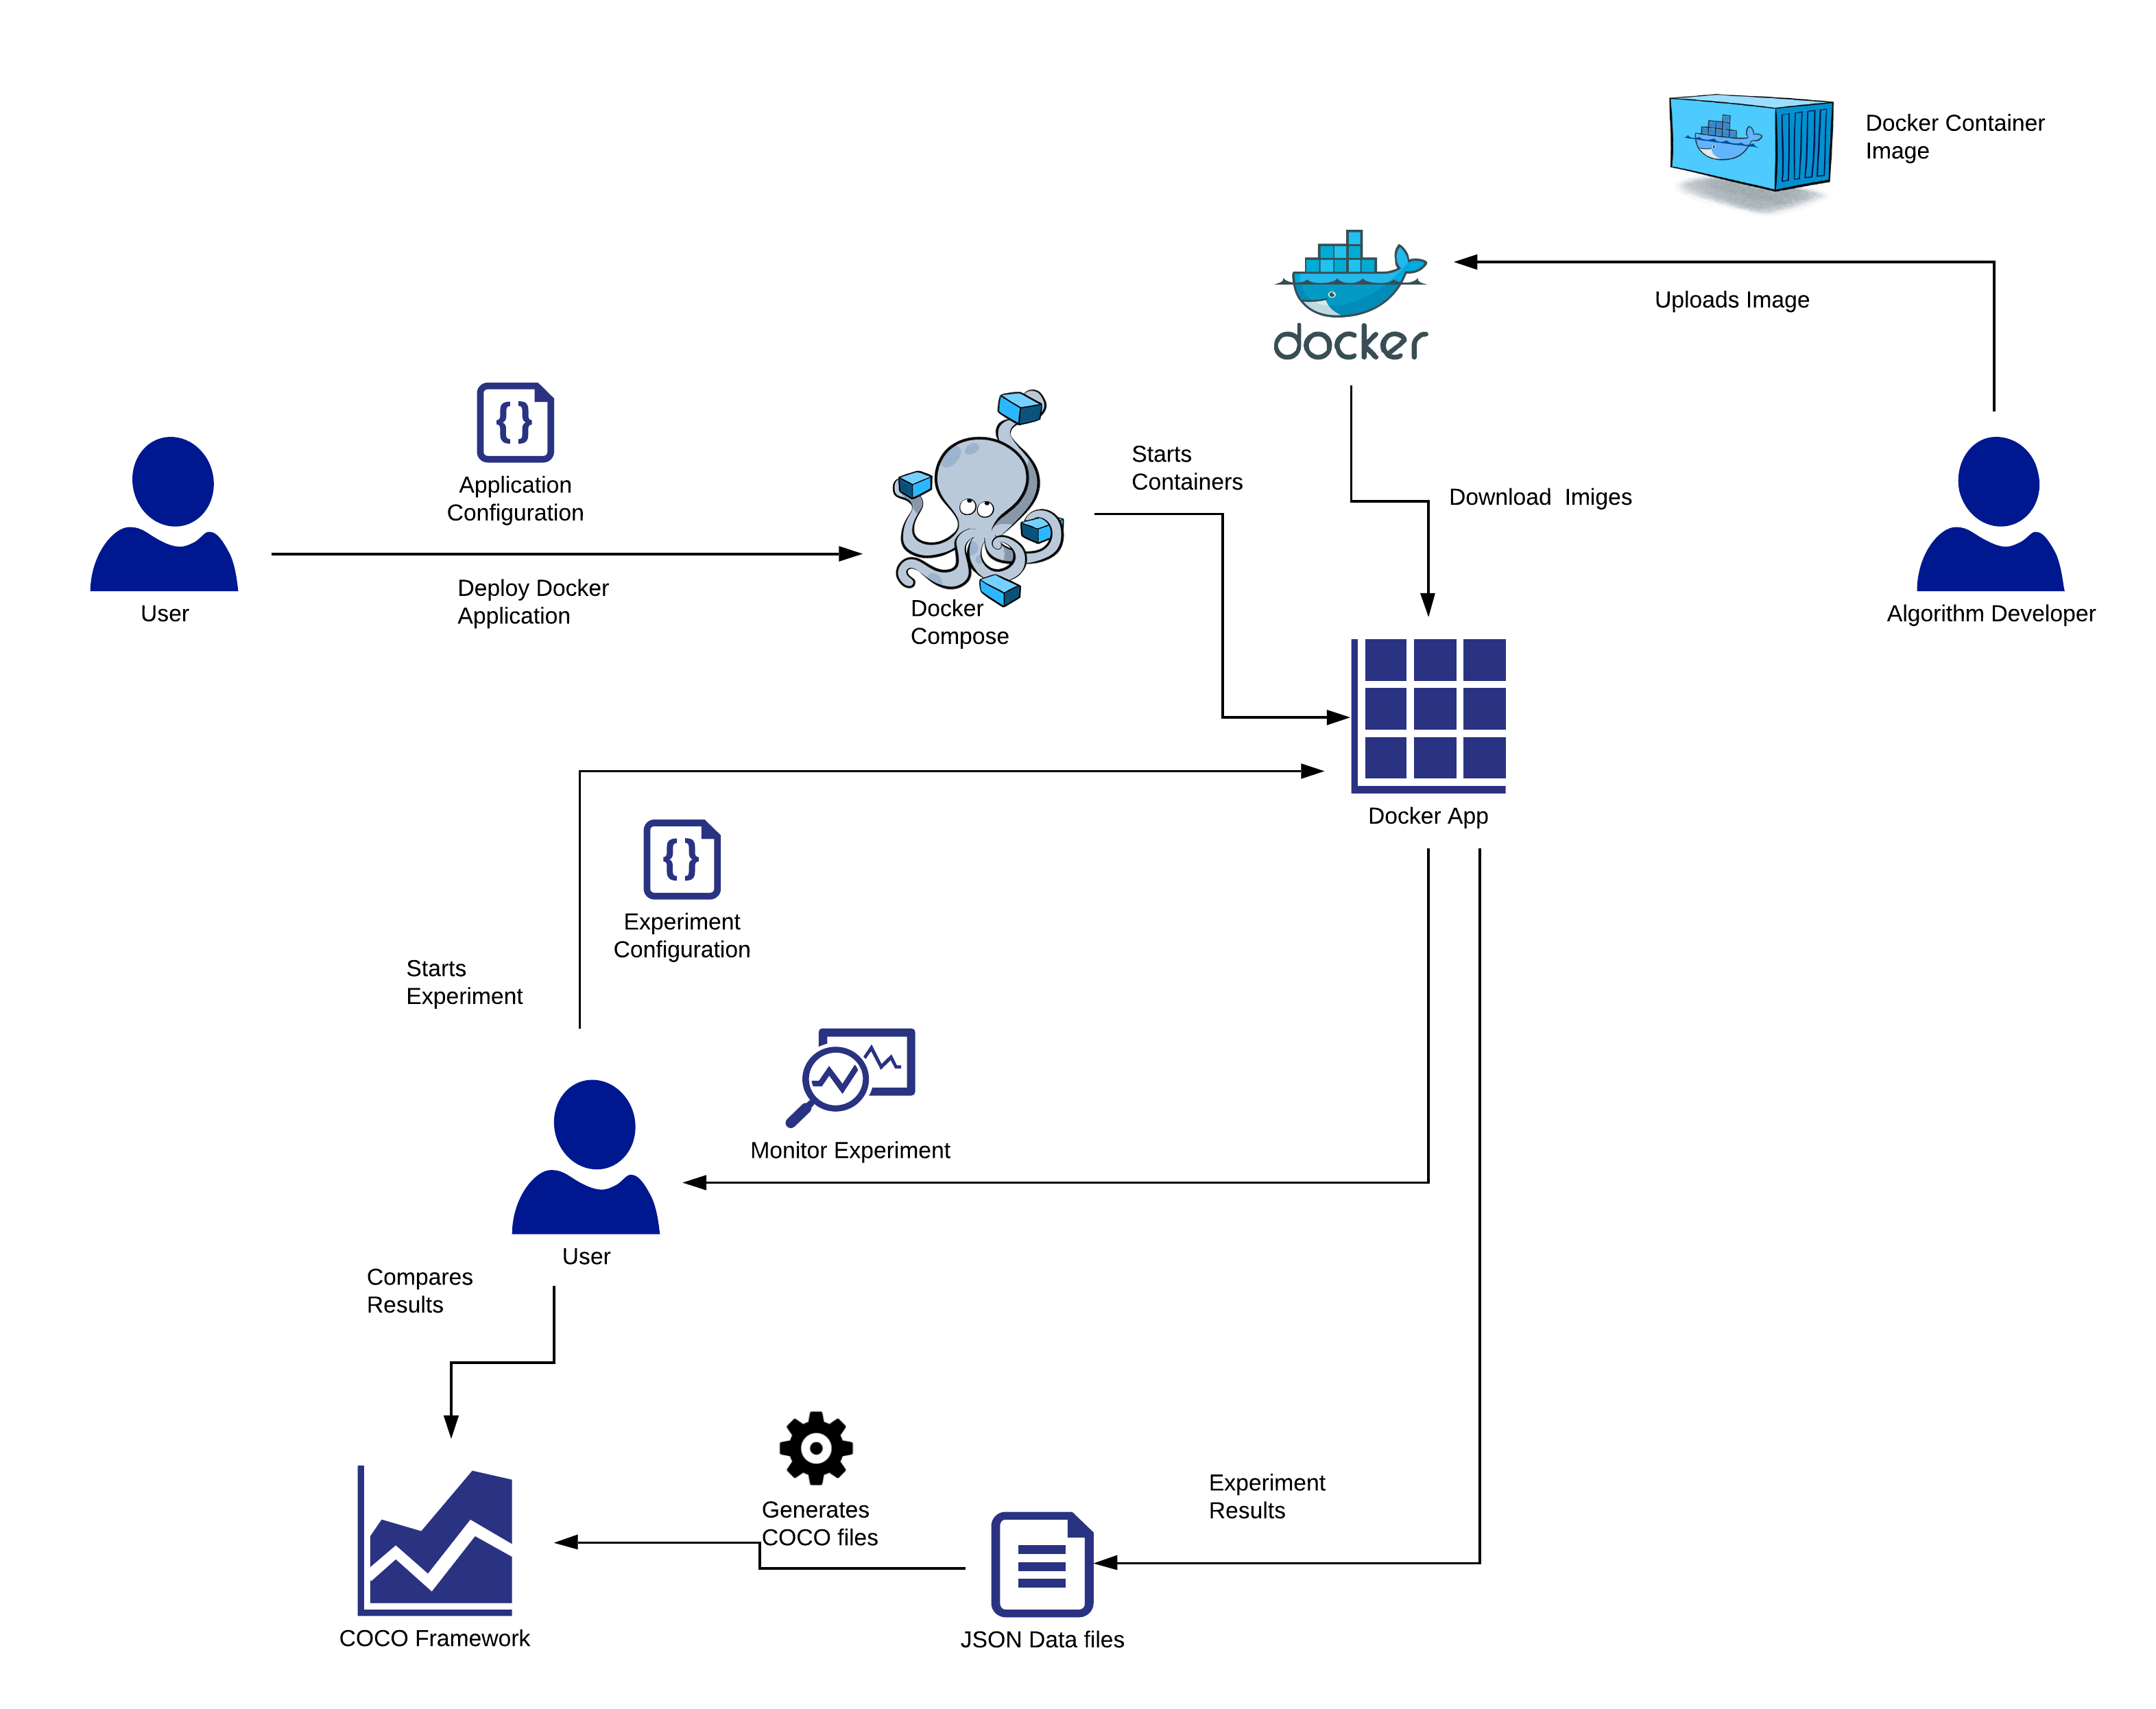
\includegraphics[width=\textwidth]{experiment_flow}
    \caption{EvoSwarm Workflow}
    \label{fig:experiment_flow}
\end{sidewaysfigure}

\subsection{EvoSwarm from the developer point of view} 

Developers can add new algorithm as stateless functions in
several ways and with two levels of integration. In the first level of
integration, the algorithm execution is not dependent on an initial
configuration created in the setup, and it only needs to take messages from the
input queue and return the modified population to the output queue. On the
second level, the algorithm receives a configuration from the initial setup,
specifying initial algorithm parameters. We show an example of the configuration
file received by workers in Figure x. % Adding to Annex or is not even needed? - M

\begin{lstlisting}[language=Python, caption=Python example]
{"problem":{
  "name":"BBOB","instance": 1,"error":1e-8,"function":4,
  "dim":3,"search_space":[-5,5],
  "problem_id":"1515-4-1-3",
  "max_iterations": 20,"population":[],
  "population_size": 100,
  "algorithm": "GA",  
  "params":{
      "GA":{"crossover": { "type": "cxTwoPoint", 
            "CXPB_RND": [0.2, 0.6], "CXPB": 0.26},
             "mutation": { "MUTPB_RND": [0.1, 0.3], 
             "indpb": 0.05, "sigma": 0.5, 
             "type":"mutGaussian","mu":0,"MUTPB":0.12},
             "selection": { 
               "type": "tools.selTournament", 
               "tournsize": 2 },
               "iterations": 50},
       "PSO": {"Vmax":5,"wMax":0.9,"wMin":0.2,
               "c1":2,"c2":2,"iterations":50 } 
    },
  "experiment":{"type":"benchmark","experiment_id": 1515}
  }
}
\end{lstlisting}


% Clarify this is the first level.
In the case of a decoupled worker, developers can implement a new stateless
Docker container that executes a daemon that continuously pulls messages from the
input queue on the Redis host specified as an environmental variable {\tt REDIS\_HOST}.
If the function is written in Python, developers can base the implementation on
the provided worker container image, adding a new type of function.  % say which function, what's its API, how can you test it - JJ
If developers use an existing library for population-based algorithms, they need
to change the standard model of execution, that first creates a random
population because, in this case, we need to start with the population provided
as a parameter. Depending on the implementation, % Depending on which implementation? - JJ
it is required to extract the
population from the JSON message and create the population object needed by the
library. Again, the state of the population must be encoded as a JSON message to
be returned as a result. Depending on the type of experiment, additional data
can be returned in the message. % how do you know the type of experiment? how do you add that? Which JSON key? - JJ
For instance, the message can include the id of
the container, or even records giving information for each iteration of the
algorithm. % Is this mandatory? Optional? How is the algorithm going to use it? - JJ
The format of the JSON message is depicted in Figure y. % Adding to Annex or is not even needed? - M
% it's probably OK if you add it, but instead of Figure it could be a listing - JJ

\begin{lstlisting}[language=Python, caption=Python example]
{
"time_stamp": 1588455316.698875,
"evals": [
  {
    "gen_num": 0, "best_fitness": -259.96925945939404,
    "best_solution": [ -4.9446848321611405, 
                        2.593007989886873, 
                        2.0011025031167673],
    "num_of_evals": 17
  },
  {
    "gen_num": 49, "best_fitness": -419.47555780783347,
    "best_solution": [ -0.9165294450108963, 
                        2.291966676472422, 
                        1.8527006568795485],
    "num_of_evals": 28
  }
],
"worker_id": "4f5eb12e-8278-40de-b0f3-4ac18171566d",
"message_counter": 1,
"message_id": "cbcd2e82-e232-4818-8aec-2cd072c7cfe9",
"best_score": -419.47555780783347
}
\end{lstlisting}

For the next level of integration, developers need to add code to the setup
container to specify additional configuration options that can be related to % related to? What do you mean here?
other workers. As with all optimization libraries, developers also need 
to write the fitness function that is going to be optimized. % Not clear how you integrate this with the rest. An example would probably help. - JJ

Migration between populations is independent of the type of algorithm, as the
controller treats messages as the same type of objects. But developers could
also change the controller to specify new rules of operation, for instance, to
change the type of migration depending on the algorithm. % Not clear how you would do this. Maybe a simple example would help - JJ

% This is the second level? - JJ
Algorithm developers can upload the container definition or images directly to
DockerHub; another option is to upload the container image definition (Dockerfile) to
GitHub and define a trigger to re-upload the image to DockerHub; this
can be defined in DockerHub (or any other registry) too.u 
% This is probably accessory. What difference would it make to upload it to GitHub?
% You also need to say in this section how it helps your overall objective. Does it contribute to reproducibility? We've talked about that elsewhere. Does it help diversity by making easy to add new algorithms? - JJ
\begin{lstlisting}[language=Python, caption=Python example]
{
 "DIM_CONFIGURATION" : 
 {
 "2":{"GEN":40,"POP_SIZE": 50,"MAX_ITER":10,"MESSAGES":10},
 "3":{"GEN":25,"POP_SIZE": 60,"MAX_ITER":20,"MESSAGES":10},
 "5":{"GEN":28,"POP_SIZE": 60,"MAX_ITER":30,"MESSAGES":10},
"10":{"GEN":50,"POP_SIZE": 70,"MAX_ITER":30,"MESSAGES":10},
"20":{"GEN":66,"POP_SIZE":100,"MAX_ITER":30,"MESSAGES":10},
"40":{"GEN":80,"POP_SIZE":125,"MAX_ITER":40,"MESSAGES":10}
},
"GA_WORKER_RATIO" : 0.5,
"FUNCTIONS": [4],
"DIMENSIONS" : [2, 3, 5, 10, 20, 40],
"CXPB_RND": [0.2, 0.6],
"MUTPB_RND": [0.1, 0.3]
}
\end{lstlisting}

\subsection{EvoSwarm Configuration} 

The administrator role is responsible for
editing the Docker Compose configuration files that reference the images created
by developers. To deploy the application, he or she needs to edit the {\tt
docker-compose.yml} file to specify the type and number of containers required
for the experiments. The {\tt docker-compose} application is responsible for
starting all the containers, and downloading new versions if it is necessary.

\subsection{Experiment Execution}

After starting the application, users can push
Experiment Definition files and start monitoring the execution in the terminal.
After the experiment is finished, the user must execute another script
that takes as argument the experiment id to generate a collection of files containing all the
data generated by the experiment in a JSON format.

\subsection{Using the COCO Framework}

Researchers can use these files to analyze and plot experiment data.  Python
scripts are included in the repository to plot the running times for the
experiments, and all other plots used in this paper;  there is also a script to
generate the files needed by the COCO framework \cite{hansen2016coco}, which can generate standard
comparisons against other methods.

\section{Experimental Setup} 
\label{setup}

We aimed to learn if the proposed solution can efficiently
improve the scalability and performance of population-based optimization
algorithms. Hence, in this section, we verify the following:

\begin{itemize}
 \item Whether we can improve the execution time of the algorithm by adding populations
 and serverless functions to the system, in particular, what is the effect of
 these changes on the scalability of the system? 
 
\item Having a multi-population enabled platform, with heterogeneous populations and
the support for mixing search strategies,  increases the performance of the
search by needing fewer function evaluations than a homogeneous setting?

\end{itemize}


To validate these questions, we used benchmark functions from the Continuous
Noiseless BBOB testbed, which is part of the Comparing Continuous Optimizers
(COCO) framework \cite{hansen2016coco}. The testbed includes 24 real-parameter,
single-objective benchmark functions, and the capability to provide additional
instances of each function. Each instance of a function has a different optimal
value. The standard benchmark of the testbed utilizes 15 instances per function
over 2, 3, 5, 10, 20, and 40 dimensions. The maximum number of Function
Evaluations (FEs) changes according to the dimension (D), and it is determined
by the expression $10^5 \cdot D$. As an example, if we have $D = 2$, the
maximum number of FEs is $200,000$


The COCO framework offers several tools to compare the performance of
algorithms, generating data sets, tables, and reports for an experiment. There
is a repository\footnote{\url{https://coco.gforge.inria.fr/doku.php?id=algorithms-bbob}} 
of more than 200 results for the noiseless BBOB testbed, collected from 
BBOB workshops and special sessions between the years 2009 and 2019. The
EvoSwarm application includes an adapted version of the noiseless BBOB testbed,
compatible with the scripts of the framework, to compare with other algorithms
in the repository.

To test the heterogeneous multi-population capabilities,  we compare the
performance between a homogeneous and an ensemble of multi-populations, using
Genetic Algorithms (GAs) and Particle Swarm Optimization (PSO). For the GA
implementation, we used the DEAP library \cite{fortin2012deap} and for the PSO,
the EvoloPy library \cite{faris2016evolopy}. Both Python libraries are
open-source. In EvoSwarm these two algorithms are implemented as stateless
functions.

Next, we show the parameters for each algorithm, with Table \ref{tab:GAparams} for
the GA and Table \ref{tab:PSOparams} for PSO. We obtained these parameters
following the same method as in a previous work \cite{garcia2017benchmarking}.
To obtain the parameters, we tested first on the Rastrigin separable function
with five dimensions. After about fifteen experiments, the most challenging
targets were achieved for this particular function. We tested again with
functions one to three, and after obtaining favorable results, the PSO and GA
algorithm parameters were set. In the GA, we randomly set the mutation and
crossover probabilities to have more heterogeneous workers; % highlight this and add citation - JJ
in these parameters,
the range of values is specified. We did not change these parameters during the
experiments, and only the population size and number of generations were
provided as parameters. 

\begin{table}
  \small
  \caption{ DEAP GA EvoWorker Parameters }
  \label{tab:GAparams} 
  \centering
  \small
  \begin{tabular}{|l|c|}
    \hline
    Selection & Tournament size=12                            \\ \hline
    Mutation & Gaussian $\mu=0.0$, $\sigma=0.5$, indbp=0.05   \\ \hline
    Mutation Probability & [0.1,0.3]                          \\ \hline
    Crossover & Two Point                                     \\ \hline
    Crossover Probability  & [0.2,0.6]                          \\ \hline
  \end{tabular}
\end{table}

\begin{table}
  \small
  \caption{ EvoloPy PSO Parameters }
  \label{tab:PSOparams} 
  \centering
  \small
  \begin{tabular}{|l|c|}
    \hline
    $V_{max}$ & 6 \\ \hline
    $W_{max}$ & $0.9$ \\ \hline
    $W_{min}$ & $0.2$ \\ \hline
    $C_1$ & 2 \\ \hline
    $C_2$ & 2 \\ \hline
  \end{tabular}
\end{table}


The experiments can be easily reproduced by using the configuration
files the the EvoSwarm application uses to run the noiseless BBOB testbed
experiments. % Specify this a bit more (with commands such as
             % docker-compose up and so on and use an itemize
             % environment to highlight it and answer to the reviewer
             % - JJ
As a first step, we must deploy the docker application using a
{\tt docker-compose.yml} file, where the number of worker containers is
specified. Then a JSON file containing the configuration parameters of the
experiment has to be provided.  Table \ref{tab:params} shows an example of these
parameters. The {\em GA-PSO Ratio} parameter indicates the proportion of
populations that will use the GA algorithm.  In the example, with a value of
$0.50$ there will be about the same proportion of GA and PSO populations. If we
specify a value of $0$, this will give us an algorithm with only PSO
populations, and finally, a value of  $1$ means that all populations will run
the GA algorithm. % Opening up the door to ask for testing with
                  % different proportion. You have to justify this
                  % value - JJ 
Next, we specify a list indicating which of the 24 benchmark
functions will be tested. In the example, the experiment will use the first five
functions.  The {\em Instances} parameter indicates how many instances of each
function will be tested. {\em Instances}  has a default value of 15. We used this
value because it is the standard for the BBOB benchmark \cite{hansen2016coco}.
In the {\em Dimensions} parameter, we define a list of the dimensions that will
be tested, and we must select additional parameters for each dimension.
According to the maximum number of function evaluations (FEs) we mentioned
earlier, we define for each dimension: the number of populations that will be
generated in the setup, and for each population,  the number of generations, and
population size. Finally, the {\em Iterations} parameter indicates how many
complete loops will be performed. All these parameters give us the maximum
number of FEs that will be performed. For instance, for $D = 2$, the maximum
number of FEs is $200,000$, which is the same as $40*50*10*10$.

\begin{table}
    \small
    \caption{ Experiment configuration example 
    }
    \label{tab:params}
    \centering
    \small
    \begin{tabular}{|l|l|l|l|l|}
      \hline
      \multicolumn{3}{|l|}{Parameter}                    & Type             & Example         \\ \hline
      \multicolumn{3}{|l|}{Worker Containers (Docker Compose)}        & \texttt{int}     & \texttt{8} \\ \hline
      \multicolumn{3}{|l|}{GA-PSO Ratio}                 & \texttt{decimal} & \texttt{0.5}    \\  \hline
      \multicolumn{3}{|l|}{Benchmark Functions}          & \texttt{list}    & \texttt{[1, 2, 3, 4, 5]} \\ \hline
      \multicolumn{3}{|l|}{Instances}                    & \texttt{integer}    & \texttt{15} \\ \hline
      \multicolumn{3}{|l|}{Dimensions}                   & \texttt{list}    & \texttt{[10, 20, 40]}        \\ \hline
      \multicolumn{3}{|l|}{Crossover Probability Range}  & \texttt{list}    & \texttt{[0.2, 0.6]}      \\ \hline
      \multicolumn{3}{|l|}{Mutation  Probability Range}  & \texttt{list}    & \texttt{[0.1, 0.3]}      \\ \hline
      \multicolumn{5}{|c|}{Dimensions}                                                      \\ \hline  
      Dimension               & Generations & Population Size & Populations  &     Iterations    \\ \hline
              10              & 50      & 140                 &      5                 & 30                \\ \hline
              20              & 66      & 200                 &      5                 & 30               \\ \hline
              40              & 80      & 250                 &      5                 & 40                \\ \hline
    \end{tabular}
\end{table}

% Section headers should be headlines. Like "Measuring scalability in
% heterogenous systems", or something like that. Experiment 1 says
% nothing about what's inside (this also applies below) - JJ
%\subsection{Experiment 1}
%\label{sec:exp1}
% Experiment 1

% What is the main objective of this experiment? Measure scalability?
% - JJ
As we mentioned before, reactive systems can scale by adding additional copies
of serverless functions. In our case, we can start additional worker containers
to have the same effect. Other authors, like Salza et al., % add
                                % reference - JJ
have used a
similar architecture, which implies that worker nodes need to have at least a certain level
of complexity, in terms of execution time,  to effectively scale on multiple
nodes, tending to linear scalability. In a population-based algorithm like
EvoSwarm, several parameters can increase or decrease the workload of workers:

\begin{itemize}
    \item The number of populations: if there are more workers than populations, workers
    must wait for work to arrive. If there are too many populations, they could be
    standing in the queue for more time.
    \item The size of populations and the number of generations:
    These parameters naturally increase the execution time.
    \item The complexity of the algorithm: For instance, in our case,
    the PSO implementation has a lower execution time than the GA.
\end{itemize}

To evaluate the effect of these parameters on the scalability of the system, we
propose  an experiment in which we selected $f_4$ (Skew Rastrigin-Bueche separable) from the
BBOB testbed. This function has been used because it is computationally demanding,
and in higher dimensions has been difficult for PSO \cite{el2009black} and GAs
\cite{nicolau2009application} to solve with the required FEs. As we
are only comparing in terms of execution time, the results from a single function
can be better understood, since there are fewer factors involved. 

We executed two sets of experiments with five and ten initial populations,
repeating each experiment using  1, 2, 4, and 8 workers.  We kept the same
maximum number of FEs, changing the relevant parameters for this. 
See Tables \ref{tab:params:10} and \ref{tab:params:5} 
for the complete list. 

\begin{table}
    \small
    \caption{Parameters used in the experiments with ten populations
    }
    \label{tab:params:10}
    \vspace{0.25cm}
    \centering
    \small
    \begin{tabular}{|l|c|c|c|c|c|c|}
      \hline
      Dimension        & 2  & 3  & 5  & 10 & 20  & 40  \\ \hline
      Generations      & 40 & 25 & 28 & 50 & 66  & 80  \\ \hline
      Population Size  & 50 & 60 & 60 & 70 & 100 & 125 \\ \hline
      Populations      & 10 & 10 & 10 & 10 & 10  & 10  \\ \hline
      Iterations       & 10 & 20 & 30 & 30 & 30  & 40  \\ \hline  
    \end{tabular}
\end{table}

\begin{table}
    \small
    \caption{Parameters used in the experiments with five populations
    }
    \label{tab:params:5}
    \vspace{0.25cm}
    \centering
    \small
    \begin{tabular}{|l|c|c|c|c|c|c|}
      \hline
      Dimension        & 2  & 3  & 5  & 10 & 20  & 40  \\ \hline
      Generations      & 40 & 25 & 28 & 50 & 66  & 80  \\ \hline
      Population Size  & 100 & 120 & 120 & 140 & 200 & 250 \\ \hline
      Populations      & 5 & 5 & 5 & 5 & 5  & 5  \\ \hline
      Iterations       & 10 & 20 & 30 & 30 & 30  & 40  \\ \hline  
    \end{tabular}
\end{table}

% 

% \subsection{Experiment 2}
% \label{sec:exp2}
% % Experiment 1

% Having a multi-population based algorithm can decrease the execution time
% because of the parallel execution of the evolution. But, having heterogeneous 
% populations might enhance evolutionary search and needless
% evaluations than homogeneous systems; heterogeneous settings, if
% done right, increases the diversity of the whole population
% \cite{araujo2008multikulti}.

% But this is a rule of thumb, and it will depend on the degree of heterogeneity,
% as well as on the algorithm itself. Some level of heterogeneity can be
% implemented by just changing the configuration parameters of each population,
% but in this case, we are interested in a heterogeneous search strategy. 
% Therefore, in this experiment we compare a multi-population with only GA and PSO populations,
% versus an ensemble of GA and PSO algorithms. We tested on the first five functions of the
% BBOB testbed. We used ten populations and eight workers for the experiment and the
% same parameters as before.  

% Shouldn't this be a subsection of experimental setup? - JJ
% \subsection{Hardware}
% \label{sec:hardware}


\section{Experimental Results} 
\label{results}

We present the results of the experiments in this section.
% The effect of a
% different number of populations on execution time is reported in  Section
% \ref{sec:exp1results}.
% The results of the performance comparison between homogeneous and
% heterogeneous search strategies are presented in Section \ref{sec:exp2results}.     
%


\begin{table}[]
    \caption{Speedup by worker and dimension, taking one worker as the baseline.}
    \label{tab:speedup-table}
    \vspace{0.25cm}
    \centering

    \begin{tabular}{c|r|r|r|r|r|r|}
    \cline{2-7}
    \multicolumn{1}{l|}{}           & \multicolumn{3}{c|}{5 Populations}                                          & \multicolumn{3}{c|}{10 Populations}                                         \\ \hline
    \multicolumn{1}{|l|}{Dimension} & \multicolumn{1}{c|}{2W} & \multicolumn{1}{c|}{4W} & \multicolumn{1}{c|}{8W} & \multicolumn{1}{c|}{2W} & \multicolumn{1}{c|}{4W} & \multicolumn{1}{c|}{8W} \\ \hline
    \multicolumn{1}{|c|}{2}         & 1.94                    & 3.12                    & 3.86                    & 1.84                    & 3.38                    & 5.98                    \\ \hline
    \multicolumn{1}{|c|}{3}         & 1.93                    & 2.77                    & 3.15                    & 1.90                    & 3.26                    & 5.96                    \\ \hline
    \multicolumn{1}{|c|}{5}         & 1.91                    & 2.90                    & 3.09                    & 1.91                    & 3.46                    & 6.14                    \\ \hline
    \multicolumn{1}{|c|}{10}        & 1.92                    & 3.03                    & 3.30                    & 1.90                    & 3.61                    & 6.41                    \\ \hline
    \multicolumn{1}{|c|}{20}        & 1.91                    & 3.14                    & 3.27                    & 1.89                    & 3.73                    & 6.71                    \\ \hline
    \multicolumn{1}{|c|}{40}        & 2.00                    & 2.92                    & 3.12                    & 1.95                    & 3.80                    & 7.52                    \\ \hline
    \end{tabular}
\end{table}


\begin{table}[]
    \small
    \caption{ Median of evaluation rate per second, for each number of workers and dimension}
    \label{tab:medians}
    \vspace{0.25cm}
    \centering

    \begin{tabular}{ccrr}
    \hline
               &         & 5 Populations    & 10 Populations \\
     Dimension & Workers & Median of rate & Median of rate  \\
    \hline
    2         & 1w      & 10,815.95      & 10,771.30      \\
    
              & 2w      & 20,704.11      & 19,197.58      \\
              & 4w      & 32,563.61      & 35,248.83      \\
              & 8w      & 40,106.09      & 59,744.88      \\
    \hline
    3         & 1w      & 9,599.62       & 9,389.69       \\
              & 2w      & 18,634.43      & 18,064.24      \\
              & 4w      & 27,607.12      & 30,419.51      \\
              & 8w      & 30,189.27      & 56,102.75      \\
    \hline
    5         & 1w      & 9,473.63       & 8,671.92       \\
              & 2w      & 18,181.18      & 16,753.68      \\
              & 4w      & 27,351.11      & 31,145.09      \\
              & 8w      & 29,257.72      & 52,985.83      \\
    \hline
    10        & 1w      & 8,353.71       & 8,145.61       \\
              & 2w      & 15,957.87      & 15,577.79      \\
              & 4w      & 25,696.70      & 29,176.94      \\
              & 8w      & 28,571.52      & 54,348.60      \\
    \hline
    20        & 1w      & 6,920.57       & 6,723.48       \\
              & 2w      & 13,297.58      & 13,136.11      \\
              & 4w      & 22,307.73      & 25,271.93      \\
              & 8w      & 24,179.41      & 46,988.12      \\
    \hline
    40        & 1w      & 5,086.88       & 4,976.05       \\
              & 2w      & 9,896.65       & 9,736.12       \\
              & 4w      & 16,326.54      & 18,695.84      \\
              & 8w      & 19,183.37      & 37,302.60      \\
    \hline  
    \end{tabular}
\end{table}


\begin{table}[]
    \small
    \caption{ Speedup of incrementing the number of workers for each dimension showing the p-rate for the Wilcoxon test}
    \label{tab:medians}
    \vspace{0.25cm}
    \centering
    \begin{tabular}{lllllll}
              &               &               & \multicolumn{2}{l}{5 Populations} & \multicolumn{2}{l}{10 Populations} \\
    Dimension & \multicolumn{2}{l}{Increment} & Speedup         & p-value         & Speedup          & p-value         \\
    2         & 1w            & 2w            & 1.94            & 6E-16           & 1.84             & 2E-16           \\
              & 2w            & 4w            & 1.61            & 2E-15           & 1.83             & 1E-15           \\
              & 4w            & 8w            & 1.24            & 1E-06           & 1.77             & 2E-16           \\
    3         & 1w            & 2w            & 1.93            & 2E-16           & 1.90             & 2E-16           \\
              & 2w            & 4w            & 1.44            & 8E-15           & 1.71             & 2E-16           \\
              & 4w            & 8w            & 1.14            & 3E-05           & 1.83             & 2E-16           \\
    5         & 1w            & 2w            & 1.91            & 9E-16           & 1.91             & 2E-16           \\
              & 2w            & 4w            & 1.52            & 3E-11           & 1.82             & 2E-16           \\
              & 4w            & 8w            & 1.06            & 5E-03           & 1.77             & 2E-16           \\
    10        & 1w            & 2w            & 1.92            & 3E-16           & 1.90             & 2E-16           \\
              & 2w            & 4w            & 1.58            & 3E-16           & 1.89             & 2E-16           \\
              & 4w            & 8w            & 1.09            & 1E-03           & 1.78             & 2E-16           \\
    20        & 1w            & 2w            & 1.91            & 2E-16           & 1.89             & 2E-16           \\
              & 2w            & 4w            & 1.64            & 2E-15           & 1.97             & 2E-16           \\
              & 4w            & 8w            & 1.04            & 1E-02           & 1.80             & 2E-16           \\
    40        & 1w            & 2w            & 2.00            & 2E-16           & 1.95             & 2E-16           \\
              & 2w            & 4w            & 1.46            & 1E-09           & 1.95             & 2E-16           \\
              & 4w            & 8w            & 1.07            & 3E-02           & 1.98             & 2E-16          
    \end{tabular}
    \end{table}


\begin{figure}[h!p]
    \centering
    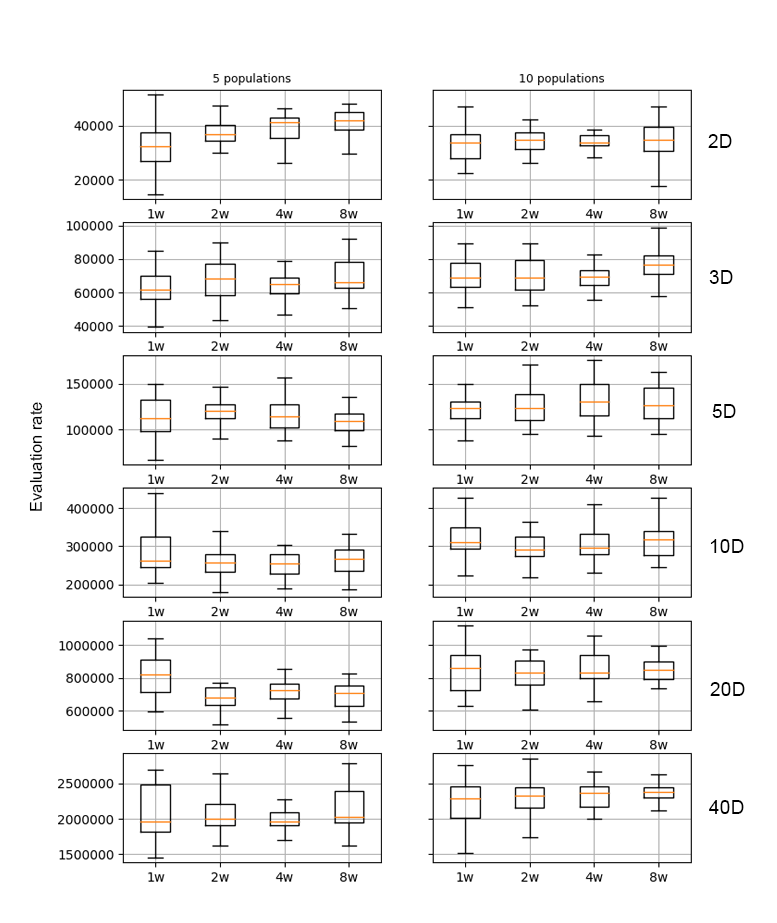
\includegraphics[width=\textwidth]{evalrate}
    \caption{Rate of number of evaluations per second, for 30 instances of the function, with different number of workers and populations sizes }
    \label{fig:spworker}
\end{figure}

\begin{figure}[h!p]
    \centering
    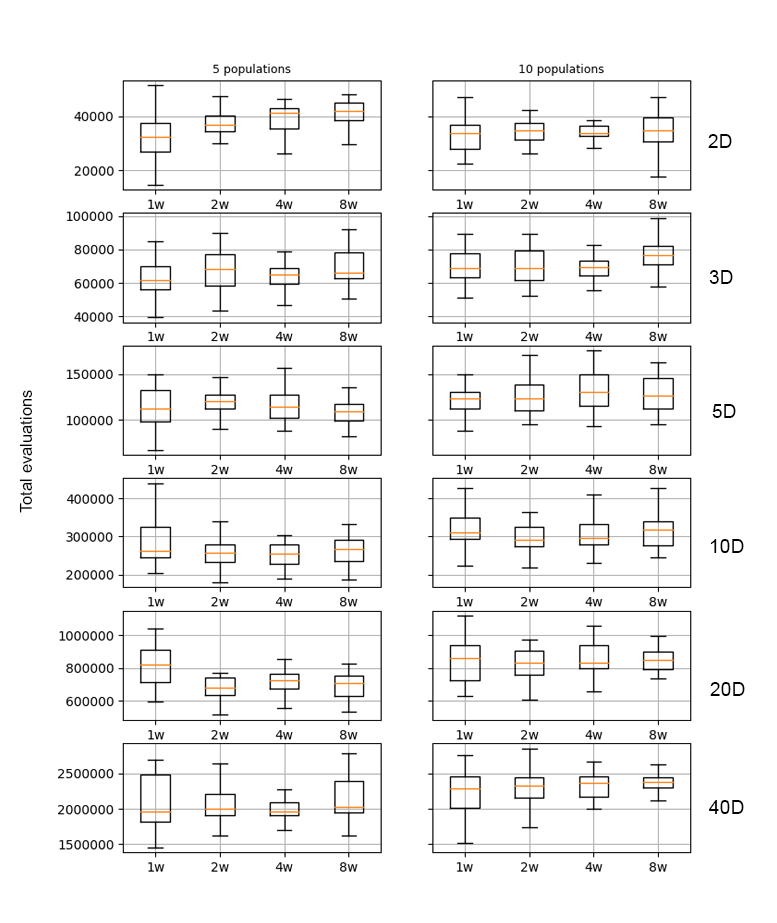
\includegraphics[width=\textwidth]{evalsworker}
    \caption{Total number of evaluations for 30 instances of the function, with different number of workers and populations sizes }
    \label{fig:spworker}
\end{figure}

%
%
% \subsection{Experiment 1}
% \label{sec:exp1results}
%
with results summarized in Figure \ref{fig:spworker}.  The
experiment consisted of executing the same benchmark on EvoSwarm twice but
changing the number of populations used in each run. This is mainly
intended as a showcase of the flexibility of the tool presented in
this paper, but we also wanted to test how the number of workers
affected the time needed to reach a solution. Adding more populations
might add more overhead, so this might have a noticeable effect.
The left column in that figure has the
results when using five populations, and the right side shows the results for
ten. In principle the main issue is how to find the right number of
workers for a particular problem, but in general we wanted to check
the communication overhead when the size of the problem increases and
how the presented framework reacted to it. % Added some explanation
% here - JJ

Charts show the execution time achieved by a certain number of
workers, for every problem dimension, which, besides, changes the
population size.
Each box-plot indicates the time required for the execution of 15 function
instances, in seconds.  Each row has a different scale on the y-axis, to
compensate for the dimension increments. It is important to notice that the
execution time can also be affected by the algorithm finding a solution with an
error smaller than the threshold, before completing all the FEs.

As expected, and in most cases, increasing the number of workers reduces the time
required for the execution of an instance, mainly when using the same parameters
(number of populations and number of workers), that is, performance
scales with the number of workers for a fixed problem and number of
sub-populations used. However, when we compare the two
options, we find some subtle differences: When using one or two
workers, using 5 populations takes less time in most cases. A 
reason for this could be that the migration of individuals takes more time to
reach the worker. For instance, when a single worker has 10 populations, only
after processing every one of them, it will start receiving mixed populations.  Although, in
all cases, and even a single worker, populations are heterogeneous, this
advantage takes more time to propagate. With four workers, almost the same
results can be achieved regardless of our selection between five or ten
populations. Also, there is not much difference between 4 and 8 workers, when
using five populations, which might indicate that some workers are
idling while populations are being processed by other workers. In
general, we can observe that keeping a ratio close to 1:1, but a bit
better than that, between the number of workers and populations, better exploits the computing
resources available. This also decreases the relation between the
overhead needed to migrate and process incoming and outgoing
population and the total computing time: more populations will need
more time to do that.

Another additional issue is related to the algorithm itself. Many more
workers than populations will have a wider range of states of
evolution in the experiment; populations that will be mixed will have
very different fitness states, which means that a part of them will
probably have been not so useful, following the intermediate
disturbance hypothesis. When the number of workers is increased, the
difference between the state of evolution of populations will be
intermediate, leading to better results; eventually, when there are as
many workers as populations, the state will be quite similar, which is
shown with a lower gap in the time won adding more workers.

\subsection{Deploying to a cloud provider}

% This is only an idea of the section
%
% First you have to say that cloud is a way of describing deployment to any kind of infrastructure in a reproducible way, and it needn't be in the cloud proper, it can be deployed to anything, that's precisely the thing. 
Several options:
    A virtual machine with a container-optimized operating system, for example,
     Google Compute Engine VMs, or Amazon EC2.  We still need to provision the
      virtual machine and run docker-compose commands as we would do in a local 
      workstation. % Remember that Salza et al. used CoreOS, which is optimized for containers - JJ
    
    A Kubernetes cluster, this provides auto-scaling and management of containerized
    application, but it needs additional configuration for provisioning. All major
    cloud-providers have Kubernetes services.

    A container orchestration service, these services are compatible with docker-compose
    files for configuration and provide transparent provisioning. Examples of these
    services are Amazon Elastic Container Service,  Red Hat Openshift, and Marantis Docker Enterprise. 

    % This is the second option. The first option was already tested, right? - JJ
As a proof-of-concept, we deployed the EvoSwarm application in Amazon Elastic
Container Service (ECS),  since it needs fewer changes in configuration (from deploying it locally using docker-compose)
and it is has a lower cost than a Kubernetes alternative.

We can define an ECS cluster directly on AWS Elastic Cloud VMs or through AWS Fargate.
Fargate is a serverless compute engine for containers that provides automatic provision 
and management of AWS ECS resources. With this service, calculating the cost of execution
is simplified because users only specify the computing units and memory for all the application,
instead of every component. 

Using the ECS CLI, we can provision a cluster with a configuration file
specifying the computing resources needed. Multicontainer applications are
% Maybe an example - JJ
deployed to ECS as tasks, and a single cluster can run multiple tasks in
parallel. When using the Fargate service as a backend, tasks are limited to a
maximum of 10 containers.  

We deployed an AWS Fargate cluster and defined a Task configuration file with
8GBs of memory and 4096 computing units, equivalent to 4 CPUs. Because of the
ten container limit, we only used seven workers and tested the same function as
in the previous experiment, but save resources only for dimensions 10 and 20.  

The results ..



\section{Conclusions} 
\label{conclusions}

In this paper we have presented the EvoSwarm framework that implements
an event-based, cloud native architecture suitable for hosting any
kind of multi-population optimization algorithm. The framework is
based in industry-standard development tools such as Docker and Docker
Compose, making easy to develop and deploy multi-algorithm distributed
experiments.

The set up of this kind of algorithms will have a big influence on the
results, since diversity is important for this kind of algorithms and
its creation and destruction play a big part of the algorithm's
performance. One of the main levers to control it in EvoSwarm is via
the number of workers that will be allocated from the beginning, which
is why we have performed an experiment mainly intended as a proof of
concept, but also devoted to show how two parameters in the framework,
number of workers and number of populations used to initially seed the
system, interact with each other. The conclusion of this experiment is
that there is an interesting interplay, with the most benefit being
obtained with a number of populations equal to the number of workers
or slightly inferior or superior, which brings algorithmic benefit
(experiment taking less time because it needs less evaluations) and
also performance benefits (experiment taking less time because
evaluations are being split between different workers.

% this is not a conclusion. The conclusion is an answer to the
% research question. This works, and works precisely for the reasons
% we say it works. - JJ
As a conclusion, EvoSwarm is a framework designed and tested according
to industry standards which is able to bring many benefits to the
bioinspired algorithm community, by showing the possibility of
creating new, high performance, mixed algorithms, which can also be
easily deployed to the cloud, or locally to systems that simply need
to have Docker and Docker Compose installed.

It also opens new possibilities. From the design point of view, it
would be interesting to try and use automatic scaling, instead of
setting the number of workers by hand. This would need a certain
amount of redesign, the most important of which would be using
container orchestration systems such as Kubernetes or Docker
Swarm. Instead of setting a fixed number of workers, only the maximum
amount would need to be established, which could be done directly or
by setting an evaluation budget.

From the algorithmic point of view, there are many possible lines of
research. Mixing population-based algorithms with other algorithms
would be a possibility, but also using different instances of
population based algorithms, such as checking how Estimation of
Distribution Algorithms would work together with evolutionary
algorithms. EvoloPy also includes other population based algorithms,
which could be tested, trying to find out which sets of algorithms are
a better match to each other. All these will be explored as future
lines of work.

\section{Acknowledgements}

This paper has been supported in part by projects TecNM-5654.19-P and DeepBio
(TIN2017-85727-C4-2-P).

\section*{References}

\bibliographystyle{elsarticle-num}
\bibliography{multipopulation}

\end{document}